\documentclass[master=elt,masteroption=eg]{kulemt}
\setup{title={Ontwerp van een RRAM geheugen voor ingebedde NV toepassingen},
  author={Wouter Diels\and Alexander Standaert},
  promotor={Prof.\,dr.\,ir.\ W. Dehaene},
  assessor={Prof.\,dr.\,ir.\,R. Lauwereins\and Prof.\,dr.\,ir.\, M. Verhelst},
  assistant={ir.\ B.~Baran \and dr.\,ir.\ S.~Cosemans}}
% De volgende \setup mag verwijderd worden als geen fiche gewenst is.
\setup{filingcard,
  translatedtitle={Design of a RRAM memory for embedded NV applications},
  udc=621.3,
  shortabstract={RRAM is een veelbelovende technologie voor het maken van embedded NV geheugens. Deze thesis behandelt het ontwerp van het leescircuit van een 1Mbit RRAM geheugen. Er wordt een geheugenarchitectuur ontworpen dat opgebouwt is uit cellen, branches, local blocks en global blocks. Hierin wordt er een uitgebreide analyse gedaan op het ontwerp en keuze van componenten zoals lastimpedantie en sense amplifier. Nadat omringende logica zoals buffers en decoders ontworpen zijn, wordt er onderzocht wat de optimale geheugenconfiguratie is. Deze optimale configuratie wordt dan onderworpen aan een speed-vdd-test en vergeleken met schakelingen in de literatuur.}}
% Verwijder de "%" op de volgende lijn als je de kaft wil afdrukken
%\setup{coverpageonly}
% Verwijder de "%" op de volgende lijn als je enkel de eerste pagina's wil
% afdrukken en de rest bv. via Word aanmaken.
%\setup{frontpagesonly}

% Kies de fonts voor de gewone tekst, bv. Latin Modern
\setup{font=lm}
\setup{inputenc=utf8}
% Hier kun je dan nog andere pakketten laden of eigen definities voorzien

% Tenslotte wordt hyperref gebruikt voor pdf bestanden.
% Dit mag verwijderd worden voor de af te drukken versie.
\usepackage[pdfusetitle,colorlinks,plainpages=false]{hyperref}
\usepackage{amsmath}
\usepackage{subfig}
\usepackage{afterpage}
\usepackage{tabularx}
\usepackage{hyperref}
\hypersetup{
    citecolor = {blue},
}
%\usepackage{showframe}

%%%%%%%

\begin{document}

\begin{preface}
  Na bijna een jaar aan deze thesis gewerkt te hebben zouden we graag een aantal mensen in het bijzonder willen bedanken voor hun hulp en steun. Ten eerste prof. Dehaene voor het onderwerp aan te bieden en toe te wijzen aan ons. Ten tweede onze begeleiders Stefan en Burak.\\
  Stefan, hartelijk dank voor de tijd die je wou vrij maken voor ons, het was heel aangenaam om een begeleider te hebben die zoveel kennis en ervaring heeft van het vakgebied.\\
  Burak, thanks for always being available for us and for providing us the resources to get our thesis underway.\\
  Verder zouden we graag Bert DeKnuydt willen bedanken voor zijn hulp met het Condor systeem. Tenslotte zouden we ook elkaar willen bedanken, we waren een goed complementair team. 
\end{preface}

\tableofcontents*

\begin{abstract}
 Nu het schalen van flash-geheugens op zijn limieten begint te stoten, is er nood aan een alternatief. Met eigenschappen zoals lage voedingsspanning, kleine geheugencel en hoge leessnelheid is RRAM één van de meest belovende kandidaten.\\\\
 Deze thesis behandelt het ontwerp van het leescircuit van een 1Mbit RRAM geheugen. De grootste uitdaging in het ontwerp van dit resistief geheugen is variabiliteit. Deze variabiliteit is kritisch op twee plaatsen: ten eerste bij de resistieve deling tussen de geheugencel en een lastimpedantie. Ten tweede bij het latchen van de sense amplifier.\\\\
 Dit werk introduceert verschillende innovaties. Zo werd er een uitgebreide analyse uitgevoerd voor de keuze van lastimpedantie. Het vormen van de referentiespanningsdistributie door middel van parallelle geheugencellen is ook een toegepaste techniek. Tenslotte wordt een analyse over de invloed van een overlappende werking van pass-gates en sense amplifier onder variabiliteit aangebracht. Verder wordt ook het ontwerp van alle andere belangrijke bouwblokken zoals decoders en buffers besproken.\\\\
 Deze kennis wordt dan gebruikt in het ontwerp van een 1Mbit geheugen in 45nm PTM technologie. Het geheugen maakt gebruik van 512 sense amplifiers die telkens gekoppeld zijn aan 2 geheugenmatrices met 32WL en 32BL. Op een voedingsspanning van 1V heeft het geheugen een random-access-leessnelheid van 435MHz. Het energieverbruik per leesoperatie bedraagt bij deze voedingsspanning 0.51pJ. Binnen de afbakening van dit werk presteert de ontworpen schakeling beter dan flash-geheugens gevonden in de literatuur.
\end{abstract}

% Een lijst van figuren en tabellen is optioneel
%\listoffigures
%\listoftables
% Bij een beperkt aantal figuren en tabellen gebruik je liever het volgende:
\listoffiguresandtables
% De lijst van symbolen is eveneens optioneel.
% Deze lijst moet wel manueel aangemaakt worden, bv. als volgt:
\chapter{Lijst van afkortingen en symbolen}
\section*{Afkortingen}

\begin{flushleft}
  \renewcommand{\arraystretch}{1.1}
  \begin{tabularx}{\textwidth}{@{}p{18mm}X@{}}
    BL & Bit Line \\
    CDF & Cumulative Distribution Function \\
    GB & Global Block \\
    HRS & High Resistive State \\
    LB & Local Block \\
    LRS & Low Resistive State \\
    MTJ & Magnetic Tunnel Junction \\
    NoBLpLB & Number of Bit Lines per Local Block \\
    NoGB & Number of Global Blocks \\
    NoWLpB & Number of Word Lines per Branch \\
    PDF & Probability Density Function \\
    PTM & Predictive Technology Model \\
    RAM & Random Access Memory \\
    RRAM & Resistive Random Access Memory \\
    SA & Sense Amplifier \\
    SL & Source Line \\
    WL & Word Line \\
  \end{tabularx}
\end{flushleft}

% Nu begint de eigenlijke tekst
\mainmatter

\chapter{Inleiding}
\label{inleiding}

Vandaag de dag is elektronica niet meer uit het leven weg te denken. Van de smartphone tot het digitaal horloge, van de boordcomputer in de moderne wagen tot de microprocessor in de vaatwasser, overal vind je wel elektronica terug.
Sinds Gordon Moore ongeveer 50 jaar geleden de uitspraak deed dat het aantal transistoren op eenzelfde oppervlakte per twee jaar zou verdubbelen \cite{Moo65}, is de industrie er over het algemeen goed in geslaagd dit te verwezenlijken. Dit leidde tot de snelle en uiterst complexe chips die we vandaag allemaal goedkoop aankopen.

Naarmate de processorkracht groter werd, steeg ook de vraag voor grotere en snellere geheugens om deze processorkracht ook effectief uit te buiten. Static Random Access Memory (SRAM) blijft een populaire keuze voor snelle ingebedde geheugens, maar heeft het nadeel vluchtig te zijn: eenmaal de voedingspanning wordt afgeschakeld, verdwijnt de informatie. Flash-geheugens, door veel mensen gebruikt voor massa-opslag in USB-sticks of SSDs, hebben ook hun weg gevonden tot het ingebedde domein en behoren wel tot de klasse van niet-vluchtige geheugens.
Het blijkt echter bijzonder moeilijk om flash-geheugens verder te verkleinen \cite{Pra10}.

Onderzoek naar nieuwe geheugens is dan ook onontbeerlijk. Zo zijn er al nieuwe nieuwe kandidaten in opmars die hoopgevende tekens geven om te concurreren met (ingebedde) flash-geheugens. MRAMs (Magnetic RAMs) en in het bijzonder STT-RAM (Spin-Transfer Torque) zullen op termijn een belangrijke rol gaan spelen.

Een andere kandidaat is Resistive RAM (RRAM of ReRAM). Daar waar SRAM- en flash-cellen de informatie bevatten via het al dan niet aanwezig zijn van lading, bevat een RRAM-cel informatie door een bepaalde elektrische weerstand aan te nemen. RRAM zou geen problemen hebben om nog even op de klassieke manier mee te schalen en is dus zonder meer een interessante piste om te onderzoeken. Bovendien zou het gefabriceerd kunnen worden met goedkopere processen dan flash-geheugens - bij flash-geheugenfabricatie zijn vaak dure extra maskers vereist.

\section{Doel en afbakening van dit werk}
Dit werk beschrijft het ontwerp van een 4MByte RRAM-geheugen voor ingebedde toepassingen. De doelstelling is een pareto-optimaal (dynamische energie-snelheid-oppervlakte) werkend circuit te ontwerpen, gewapend tegen variabiliteit - ongecorreleerde gedragsvariaties van componenten. Het ontwerp houdt rekening met data-retentie bij het uitlezen van bits. De analyse focust op de leesbewerking, de schrijfbewerking valt buiten het bereik van dit werk. [Er worden wel mogelijke oplossingen aangereikt, maar deze werden niet uitdrukkelijk onderzocht]

Voor de leesbewerking wordt het geheugen-element gemodeleerd als een weerstand waarvan de nominale weerstandswaarde afhangt van de celtoestand. Wanneer variabiliteit wordt onderzocht, zal deze weerstandswaarde een stochastische variabele worden met een normale verdeling.

Temperatuursvariaties werden niet in rekening genomen, maar aangezien dit een globale variabele is en het systeem differentieel werkt, wordt niet verwacht dat de performantie aanzienlijk zal verminderen.

Alle data die worden getoond, komen voort uit Spectre-simulaties met 45nm PTM transistormodellen.

\section{Structuur van de tekst}
In hoofdstuk \ref{cell} zal de technologie van een RRAM geheugen uiteengezet worden, alsook diens toepassingen. Ook zal het elementaire principe om uit een weerstand een nuttig elektrisch signaal te vormen uitgelegd worden. In hoofdstuk \ref{architecture} wordt het geheugensysteem vanuit vogelperspectief besproken. Er wordt hier ook aangehaald wat de tunebare parameters zijn van de architectuur. Voor een robuuste, snelle en laag-energetische leesoperatie uit te voeren is het belangrijk het geheugenelement te combineren met een zorgvuldig gekozen impedantie, dit wordt onderzocht in hoofdstuk \ref{loadanalysis}. Uiteindelijk zal er een bitstream moeten gegenereerd worden aan de uitgang van het systeem, de sense amplifier zorgt hiervoor en wordt besproken in hoofdstuk \ref{sensamp}.
In de geheugenstructuur zijn ook bepaalde logische (digitale) operaties nodig om op basis van het opgegeven adres de juiste cel aan te spreken, de hiervoor gebruikte blokken worden beschreven en geanalyseerd in hoofdstuk \ref{periphery}.
Ten slotte zal in hoofdstuk \ref{timing-optimization} de timing van controlesignalen onderzocht worden en hoe het systeem te optimaliseren door middel van de architectuurparameters te tunen.
\chapter{Geheugencel}
\label{cell}
Elk geheugen bestaat uit een verzameling individuele cellen die op een of andere manier informatie bevatten.
In dit hoofdstuk wordt eerst dieper ingegaan op de manier waarom een R-RAM geheugencel informatie bevat en vervolgens hoe deze informatie [elektrisch] kan worden uitgelezen.

\section{Memristor}
Het essentiële element van een R-RAM geheugencel is ontegenspreekbaar de zogenaamde memristor.
De memristor wordt ook wel gezien als de 4\textsuperscript{e} passieve component, naast de weerstand, spoel en condensator.

\subsection{Theoretisch principe}
In 1971 publiceerde Leon Chua een artikel waarin hij opmerkte dat er voor de 4 fundamentele circuitvariabelen (de spanning v, stroom i, lading q en fluxbinding $\lambda$\footnote{$\lambda(t) =  \int^{t}_{-\infty} v(\tau) \, d\tau $, voor een ideale inductantie is dit hetzelfde als magnetische flux: $\lambda = \phi$ }) van 6 mogelijke onderlinge relaties er slechts 5 gekend waren: $q(t) =  \int^{t}_{-\infty} i(\tau) \, d\tau $, $\lambda(t) =  \int^{t}_{-\infty} v(\tau) \, d\tau $, $v(t)=R*i(t)$, $q(t)=C*v(t)$ en $\lambda(t) = L*i(t)$ volgen uit de wetten van Maxwell en uit de definities van de weerstand, spoel en condensator, maar er ontbrak een relatie tussen $\lambda$ en q.\cite{Chu71} Hij suggereerde dat er een 4e nog niet ontdekte passieve 2-pool moest bestaan die dit verband herbergde.
Uit zijn wiskundige berekeningen kwam hij tot de conclusie dat deze component zich ogenblikkelijk als een weerstand zou gedragen, maar dat de weerstandswaarde verandert aan de hand van het verloop van de stroom in de tijd. Gebaseerd op deze conclusie doopte hij deze component de memristor (een contractie van memory en resistor).

\subsection{Fysische werking}
Chua beëindigde zijn artikel met te erkennen dat er op dat moment nog geen fysische memristor was ontdekt, maar dat dit in de toekomst wel kon gebeuren, al dan niet zelfs per ongeluk. Hij gaf zelfs aan dat er misschien al in die tijd materialen met memristorkarakteristieken gebruikt werden, maar dat men hier over keek. Hij zou gelijk krijgen.


\subsection{Toepassingen}


\section{Memristor in een geheugenstructuur}

In dit werk wordt gebruik gemaakt van een \emph{1 Transistor, 1 Resistor} (maar eigenlijk dus een memristor) architectuur, de combinatie van deze twee vormt de geheugencel, maar er zijn nog een paar andere configuraties die zouden toegepast kunnen worden.

\subsection{1T1R}

\subsection{1R}

\subsection{1T1D}



\section{Besluit}


\chapter{Geheugenarchitectuur}
\label{architecture}
De afzonderlijke geheugencellen zullen samengebracht worden in een geheel.
Dit hoofdstuk bespreekt de algemene structuur alsook de vrijheidsgraden die in hoofdstuk \ref{timing-optimization} onderzocht worden om tot een optimaal werkend systeem te komen. Ten slotte zullen ook nog de bouwblokken aangekaart worden die meer uitvoerig besproken worden in de volgende hoofdstukken. 


\section{Cel}
Zoals besproken in hoofdstuk \ref{cell} is dit het bouwblok dat het vaakst terug te vinden is in het geheugensysteem.
De cel bestaat uit een memristor en een transistor (1T1R-cel). De geheugencel heeft drie terminals: de gate van de transistor, die verbonden wordt met een wordline, de source van de transistor, die verbonden wordt met een sourceline en tenslotte de terminal van de memristor, die verbonden wordt met een bitline.
%Een cel waarvan memristor zich in een willekeurige resistieve staat bevindt is een datacel, terwijl de memristor van referentiecellen in een voorgeprogrammeerde en dus gekende resistieve staat verkeert.

\section{Branch}
In een branch worden er een bepaald aantal datacellen verbonden aan één BL en één SL. Dit aantal wordt \emph{Number of Word Lines per Branch} (NoWLpB) genoemd en is een van de vrijheidsgraden van de geheugenarchitectuur. Naast alle datacellen is er ook nog één referentiecel - dit zijn cellen waarvan de resistieve staat voorgeschreven is - verbonden aan de BL en SL van de branch.
Elke BL wordt via een pMOS-transistor (al dan niet met nog een impedantie tussenin) gekoppeld aan de voedingspanning Vdd en via een nMOS-transistor aan de grondspanning Vss. In dit werk is er enkel een nMOS-transistor die de SL verbindt met Vss.\footnote{In een volledig geheugensysteem zou de SL via een pMOS ook nog verbonden zijn met een niet onderzochte spanningsknoop Vdd\_write. De pMOS zou dan worden aangezet voor schrijfwerking.} De nMOS-transistoren aan BL en SL fungeren als schakelaars, de pMOS-transistor wordt daarenboven ook gebruikt als impedantie voor een resistieve spanningsdeling (zie hoofdstuk \ref{loadanalysis}).
Ter illustratie wordt de samenhang tussen cel en branch getoond in figuur \ref{fig:cellbranch}.

\begin{figure}
  \centering
  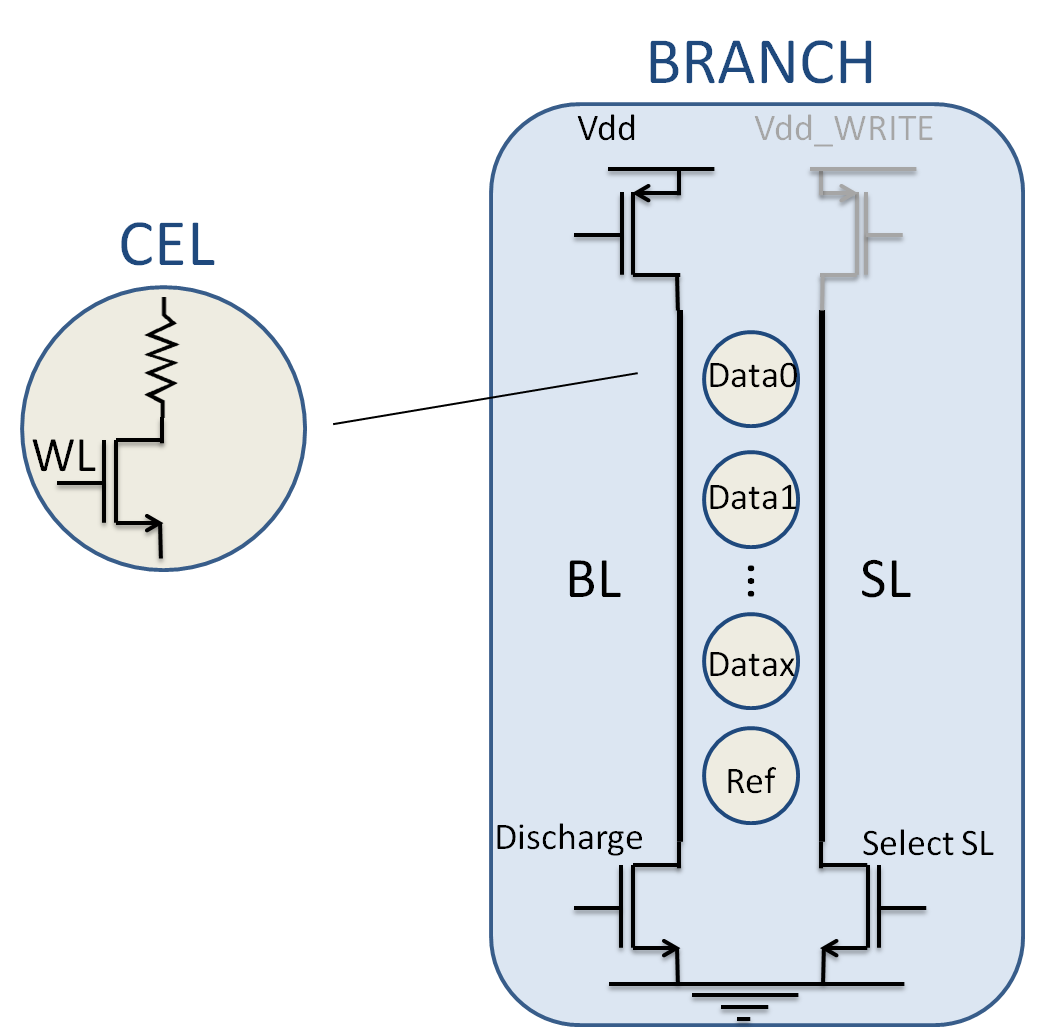
\includegraphics[scale=0.3]{../fig/hfdstk-architecture-cell-branch.png}
  \caption{Een geheugencel en een branch}
  \label{fig:cellbranch}
\end{figure}

\section{Local Block}
Verschillende BLs en SLs worden samengebracht in een local block, waarvan de vrijheidsgraad \emph{Number of BitLines per Local Block} (NoBLpLB) heet. In een LB bevinden er zich dus NoBLpLB x NoWLpB datacellen en NoBLpLB referentiecellen. Ook bevat een local block zowel BL- als WL-decoders. De afzonderlijke BLs worden via passgates verbonden tot een uitgangsknooppunt.
De structuur van een local block is geïllustreerd op figuur \ref{fig:LB}.
De uitgangen van de WL-decoder sturen de data-WLs aan [eventueel met een buffer], de uitgangen van de BL-decoder activeren een spanningsdeling op de BLs.\footnote{Indien schrijfwerking zou toegevoegd worden, zouden de uitgangen van de BL-decoder aan twee AND-poorten worden verbonden; bij leesoperatie brengt de uitgang van de ene AND-poort de resistieve deling op de BL teweeg, bij schrijfoperatie zet de uitgang van de andere AND-poort een pull-up-operatie van de BL naar Vdd\_write op.} De referentie-WL is via een extern signaal verbonden. Voor een gedetailleerdere beschrijving over hoe de decoderuitgangen gebruikt worden, zie sectie \ref{timing}.
Aangezien een LB zowel data- als referentiecellen bevat, gaat een LB twee werkingsmodes hebben: een mode waarbij er één datacel wordt aangesproken en een mode waarbij er een bepaald aantal referentiecellen in parallel wordt aangesproken.
Figuur \ref{fig:LB-details} geeft een meer gedetailleerd beeld van een LB, decoders weggelaten.

\begin{figure}
  \centering
  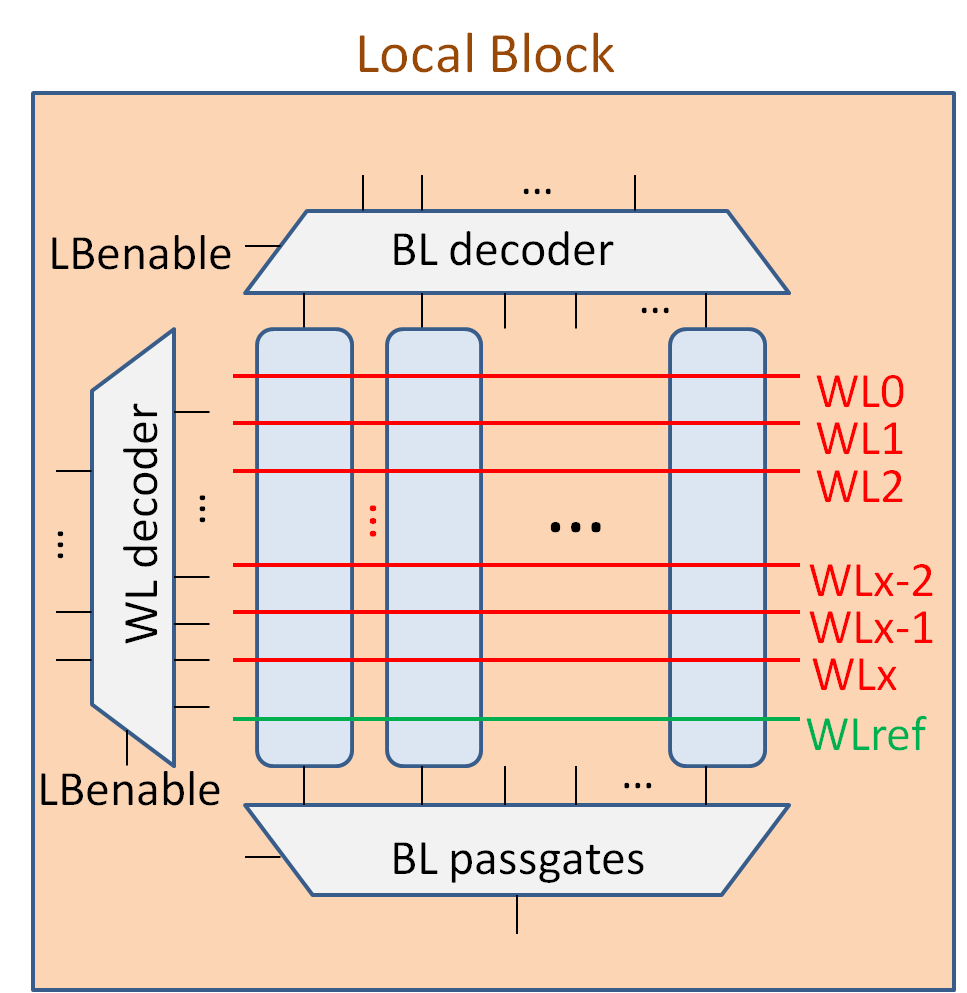
\includegraphics[scale=0.3]{../fig/hfdstk-architecture-localblock.png}
  \caption{Een Local Block}
  \label{fig:LB}
\end{figure}

\begin{figure}
  \centering
  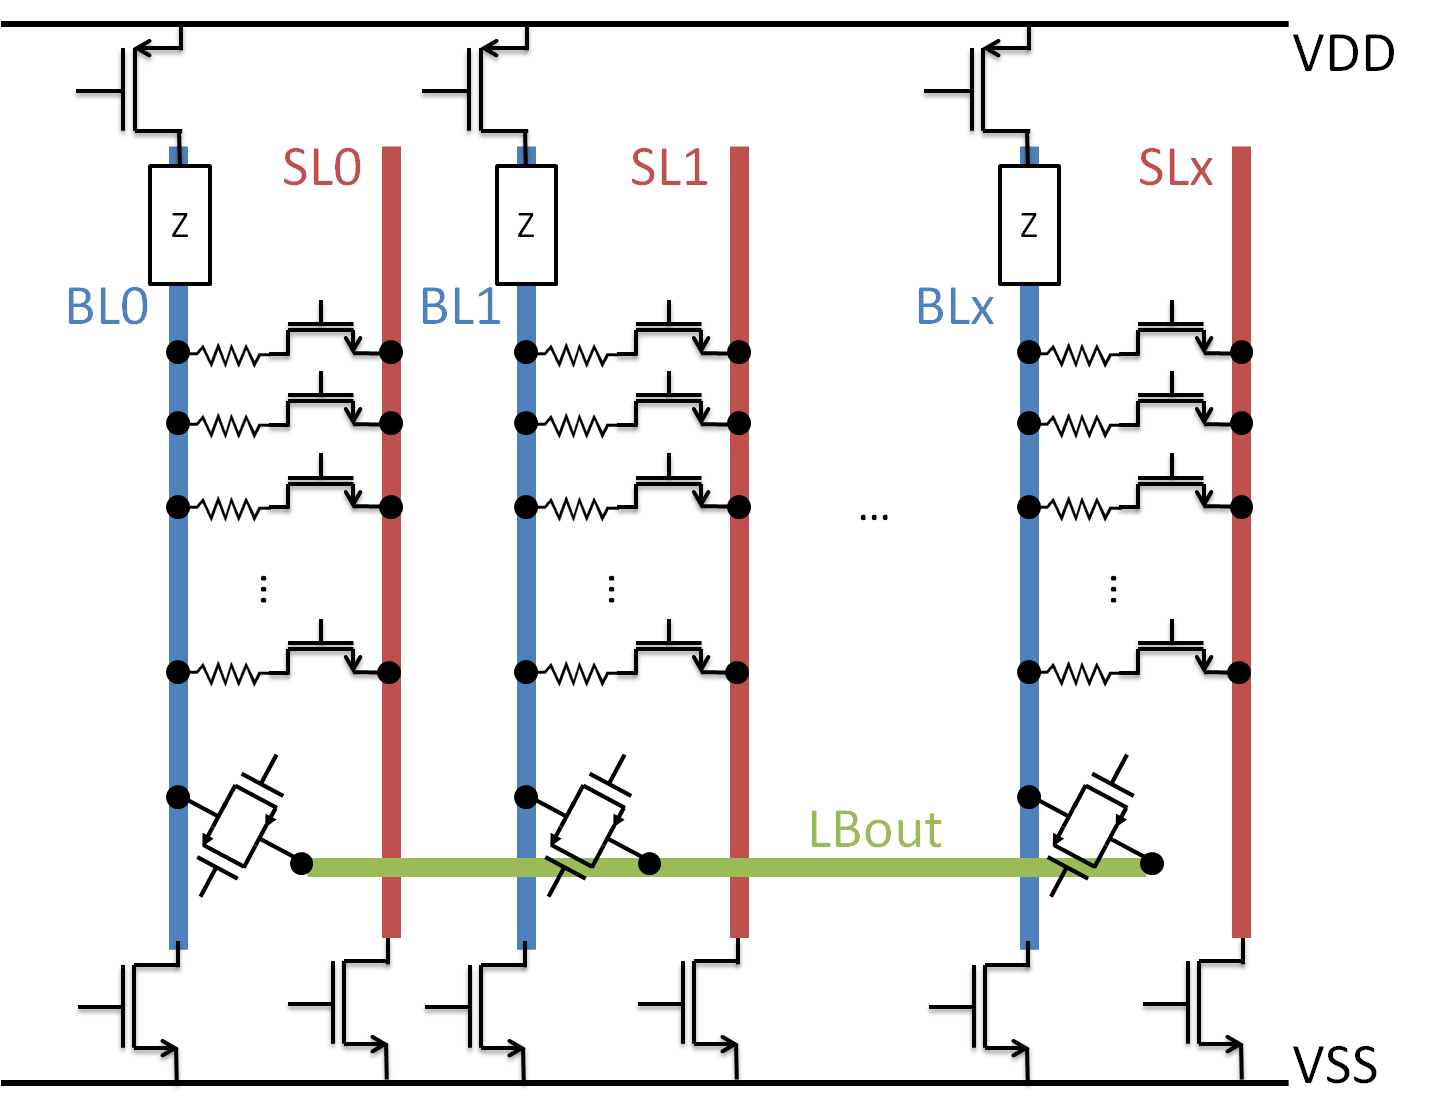
\includegraphics[scale=0.3]{../fig/hfdstk-architecture-LB-details.png}
  \caption{Een meer gedetailleerde illustratie van een LB, decoders zijn weggelaten}
  \label{fig:LB-details}
\end{figure}

\subsection{Datasignaal uitlezen}
Het datasignaal is de spanning op de BL nadat er een resistieve deling is gebeurd, waarbij er stroom vloeit door één cel. De last die hangt aan de voedingsspanning, op figuur \ref{fig:dataread} voorgesteld als een pMOS-transistor, wordt aangeschakeld, alsook de nMOS-transistoren in de cel en aan de sourceline. Er vloeit een stroom langs dit pad: I=Vdd/Rtot, en de spanning op de BL is V=IReq. Om dit datasignaal op de uitgangsknoop van het LB te krijgen, wordt de bijhorende passgate van de BL in kwestie geactiveerd.

\begin{figure}
  \centering
  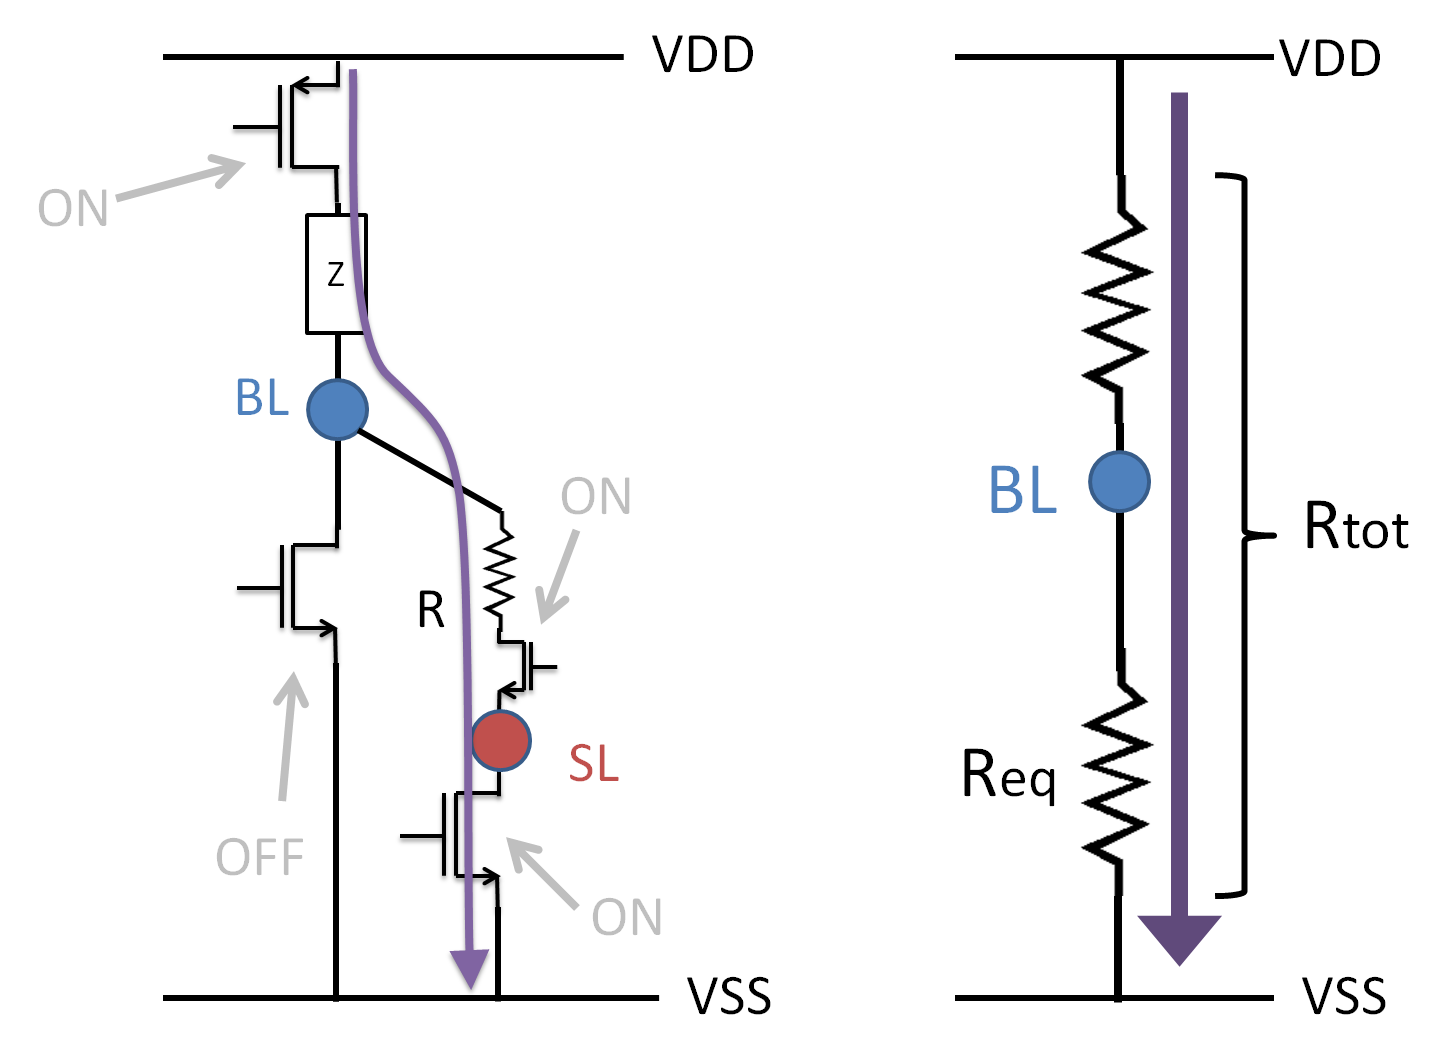
\includegraphics[scale=0.3]{../fig/hfdstk-architecture-datasignal.png}
  \caption{Methodologie om datasignaal te verkrijgen op een BL}
  \label{fig:dataread}
\end{figure}

\subsection{Referentiesignaal uitlezen}
Het referentiesignaal is een spanning die tussen de spanning van een lage resistieve datacel en een hoge resistieve datacel moet liggen. Een dergelijk signaal kan verkregen worden door twee BLs kort te sluiten zoals op figuur \ref{fig:2cellref}. In dit ontwerp zal de kortsluiting gerealiseerd worden door de passgates van de BLs aan te zetten, zo komt het referentiesignaal bovendien ook op de uitgangsknoop te staan. In theorie is het voldoende om 2 BLs [de ene met een HRS cel en de andere met een LRS cel] kort te sluiten om het referentiesignaal te verkrijgen. Er zit echter op de resistieve geheugenelementen variabiliteit: er wordt aangenomen dat $R_{H}$ normaal verdeeld is met $\mu = 32500\Omega$ en $\sigma = 833\Omega$. $R_{L}$ is ook normaal verdeeld met $\mu = 7500\Omega$ en $\sigma = 833\Omega$. Dit betekent dat ook de data-signalen en referentie-signalen stochastische variabelen zijn.
Door echter steeds meer referentiebitlijnen kort te sluiten gaat de spreiding van het referentiesignaal dalen [maar gaat het energieverbruik stijgen]. Bovendien kan men de verwachtingswaarde verschuiven door meer HRS (LRS) referentiegeheugenelementen te gebruiken dan LRS (HRS).

\begin{figure}
  \centering
  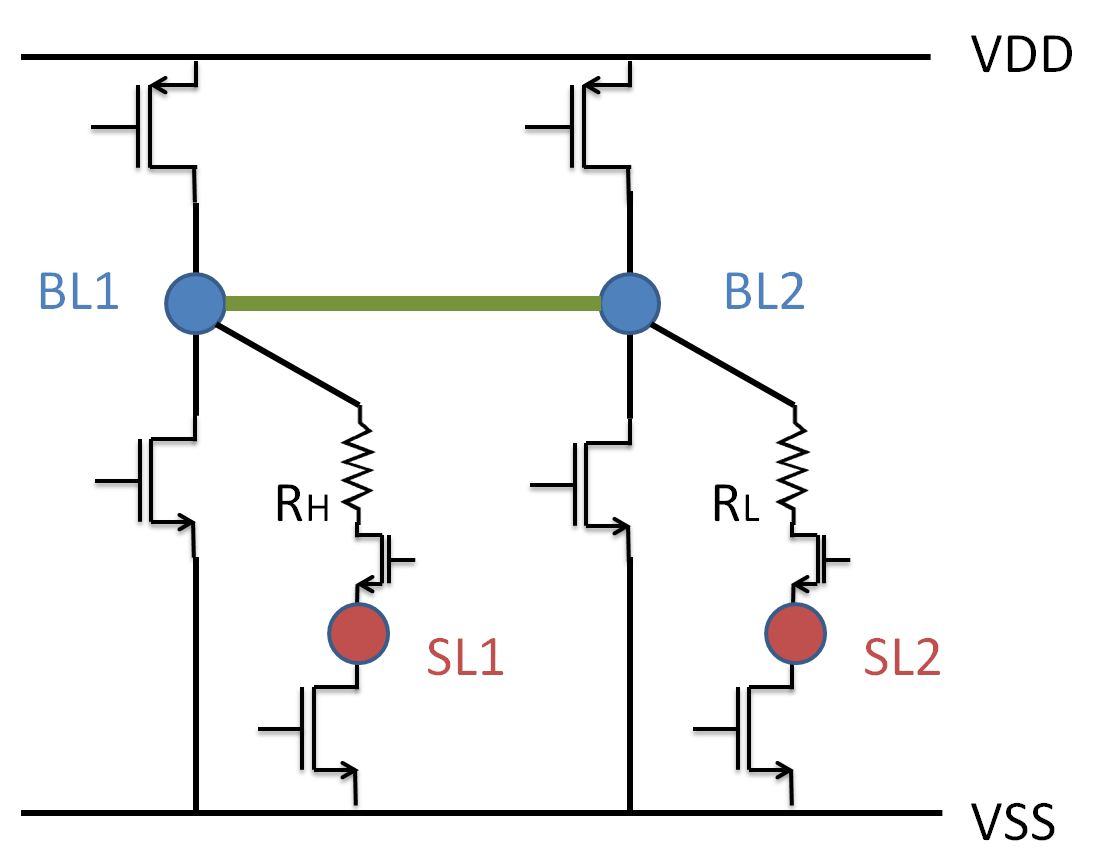
\includegraphics[scale=0.3]{../fig/hfdstk-architecture-ref2cell.png}
  \caption{Topologie om referentiesignaal te verkrijgen}
  \label{fig:2cellref}
\end{figure}

\section{Global Block}
\label{globalblock}
Een global block bestaat uit twee LBs en een sense amplifier (SA) met bijhorende sample-and-hold-schakelaars (S\&H). In het ene LB gaat er een datasignaal geproduceerd worden, in het andere een referentiesignaal (zie figuur \ref{fig:GB}. Vervolgens gaat de SA dit kleine signaalverschil versterken tot een zuivere rail-to-rail output.
Aan de uitgang van het GB verschijnen dan ook de opgevraagde bits.
De laatste architectuurvrijheidsgraad is de \emph{Number of Global Blocks} (NoGB), het totale geheugen bevat dus NoGB x 2 x NoBLpLB x NoWLpB datageheugencellen.

\begin{figure}
  \centering
  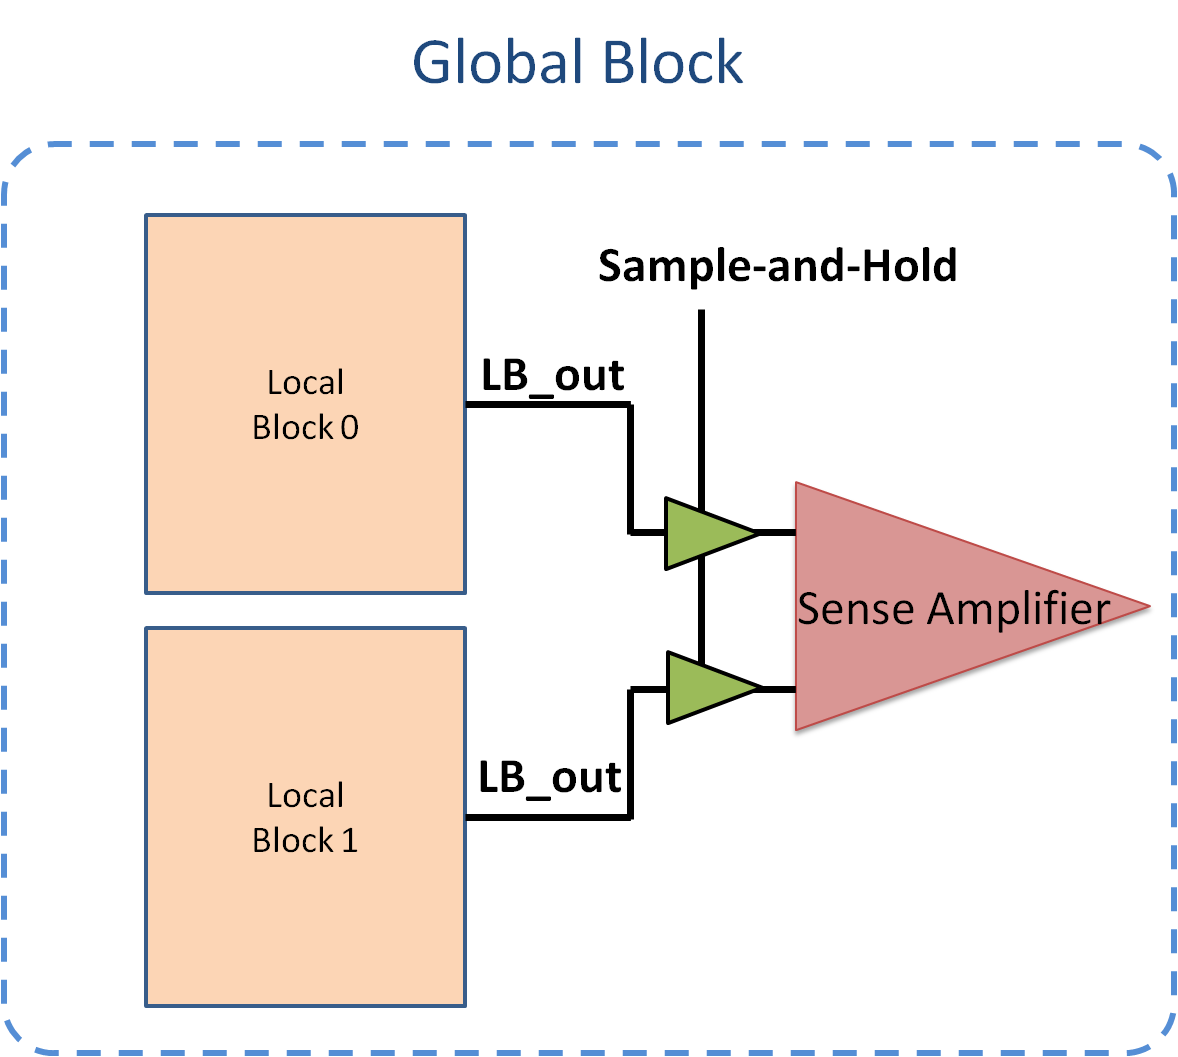
\includegraphics[scale=0.3]{../fig/hfdstk-architecture-globalblock.png}
  \caption{Een Global Block}
  \label{fig:GB}
\end{figure}

\section{Besluit}
De geheugenarchitectuur werd in vogelvlucht overlopen. De kleinste bouwblok is de cel, deze wordt geplaatst in een branch. Verschillende branches vormen samen een local block, dat ook decoders en multiplexers bevat. Twee local blocks en een sense amplifier met bijhorende passgates worden gegroepeerd tot een global block. Het totale geheugen bestaat tenslotte uit een verzameling global blocks.


\chapter{Lastimpedantie-analyse}
\label{loadanalysis}
Om een cel uit te lezen wordt er een spanning gegenereerd op de bitline door middel van een spanningsdeling.
Het is dus belangrijk om de 2 impedanties van de spanningsdeler zodanig te kiezen voor optimale snelheid, bitline spanningsverschil en spanningsval over de memristor.
Ook belangrijk is dat deze impedanties robuust zijn tegen variabiliteit.

\section{algemene last eigenschappen en specificaties}\label{sec:simplemodel}
In deze eerste sectie bestuderen we de combinatie van last en memristor cell als een heel simpel model namelijk twee weerstanden in serie (zie figuur \ref{fig:simplemodel}). Dit om aan te tonen dat de weerstands waarde van de last een grote invloed heeft op de het voltageverschil tussen een hoge en lage cel weerstand, bitlijn snelheid en de sensitivity van beide.
Het verschil in bitlijn voltage tussen een hoge en lage cell is van belang voor de toleraties op de referentie voltage en sense amplifier mismatch. In het simple model kan het verschil in bitlijn voltage analitisch berekend worden met de volgende formule:
\begin{equation}
 \Delta V = \frac{R_{HRS}}{R_{last}+R_{HRS}} - \frac{R_{LRS}}{R_{last}+R_{LRS}}
\end{equation} 
Voor constante waarden van $R_{HRS}$ en $R_{LRS}$ zal er een maximum zijn in $ \Delta V$ zoals duidelijk gezien kan worden in figuur \ref{fig:rpiek}. De sensitiviteit van de last weerstand op het spanningsverschill, moet men voorzichtig interpreteren. Op figuur \ref{fig:rpiek} kan gezien worden dat de helling voor de piek stijler is als na de piek. Het is dus beter om een iets grotere weerstand te hebben als een iets te kleine weerstand. Maar als men de weerstand naar transistor afmetingen vertaalt, kan met dit op verschillend manieren realiseren. Een grote weerstand realiseren met een transistor met minimale lengte, zal betekenen dat de breete van de transistor klein moet zijn. Dit zal dan gevoeliger zijn voor mismatch dan een grotere breete van transistor.\\
De snelheid van het opladen van de bitlijn kan in het simple model ook analitisch geschreven worden. De volgende vergelijking stelt de tijd voor waar de bitlijn $99\%$ is opgeladen.

\begin{align}
t = -ln(0.01)*RC\\
R^{-1} = \frac{1}{R_{cell}} + \frac{1}{R_{last}}
\end{align}

Deze tijd zal kleiner worden als de R kleiner word, dit vertaalt zich dan naar een kleine last weerstand.

\begin{figure}[!ht]
\centering
\subfloat[het simpel bitlijn model]{ 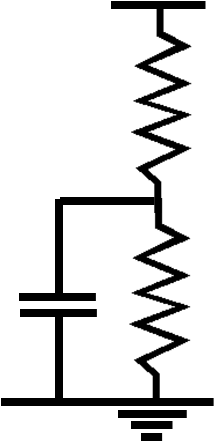
\includegraphics[width=0.20\textwidth] {../fig/hfdst-last-simplemodel.png} \label{fig:simplemodel}}
\subfloat[Verschil in Bitlijnspanning in functie van lastweerstand]{ 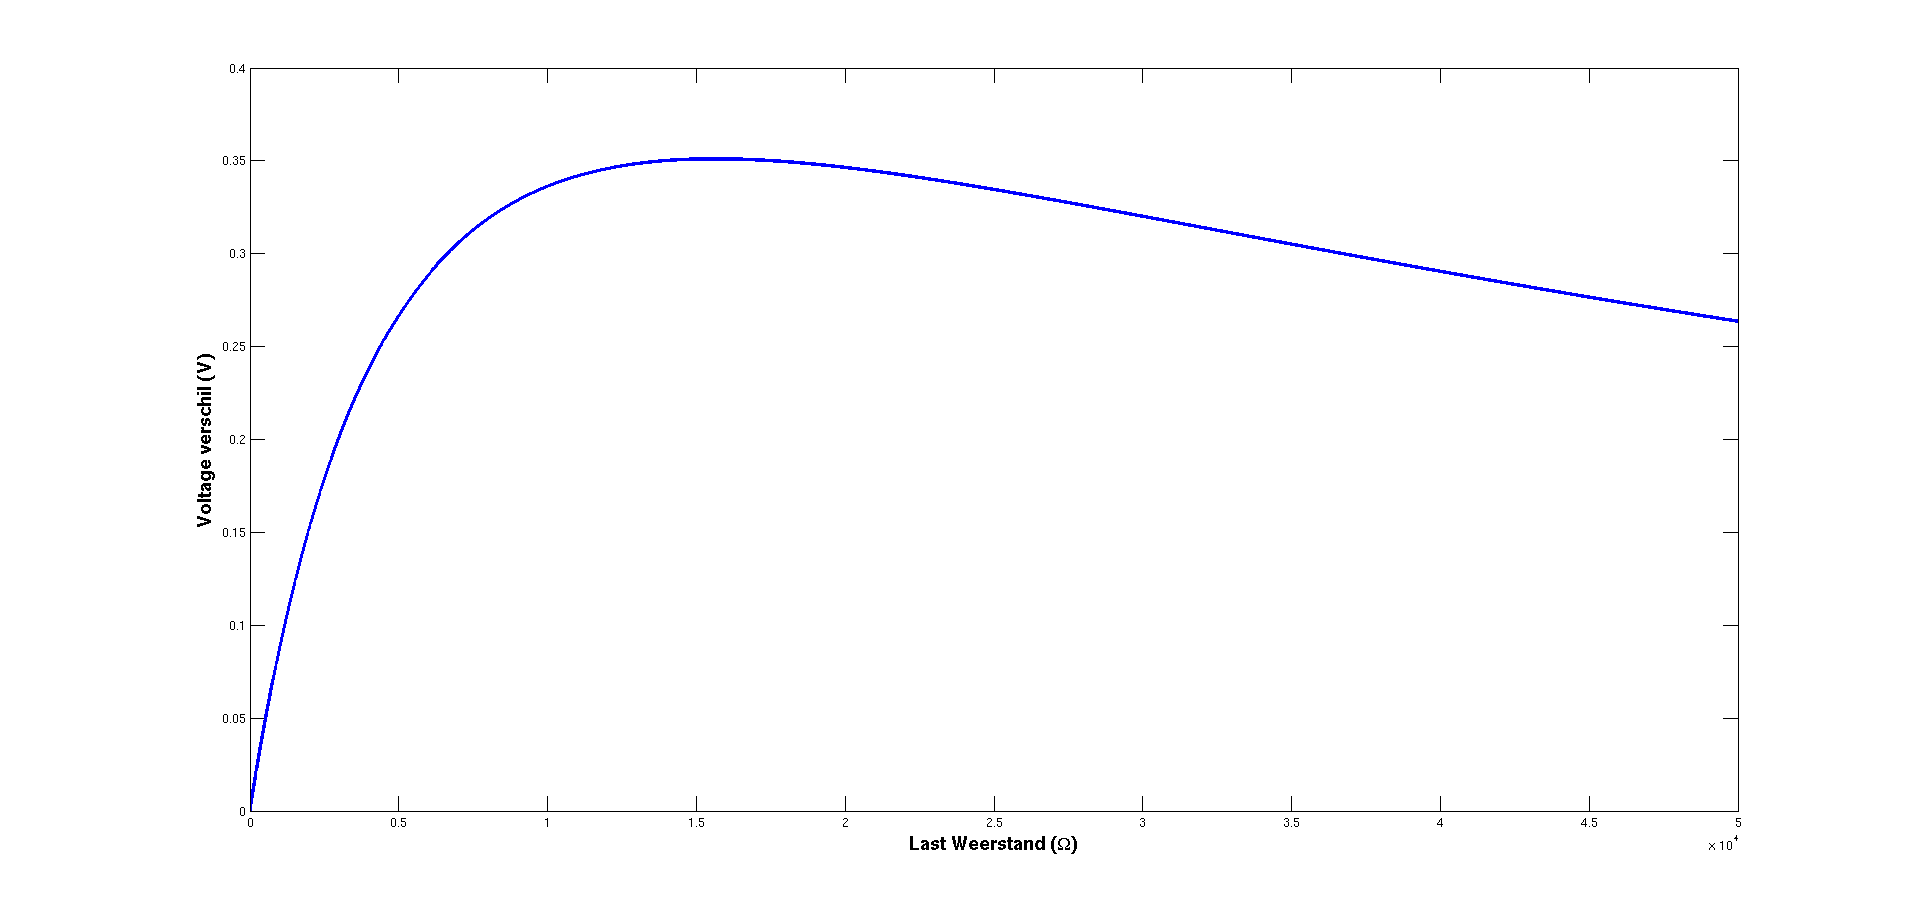
\includegraphics[width=0.80\textwidth] {../fig/hfdst-last-rpiek.png} \label{fig:rpiek}}
\caption{}
\end{figure}




\section{evalueren van de last}
Om verschillende lasten met elkaar te kunnen vergelijken, is het belangrijk om hun eigenschappen allemaal op dezelfde manier te bekomen. Figuur \ref{fig:simsetup} geeft de verschillende aspecten van de gebruikte simulatie setup weer. Het test circuit (Figuur \ref{fig:simcircuit}) stelt een bitlijn voor met een capaciteit van 18fF, wat ruiw weg overeenkomt met een bitlijn met 100 cellen op. Aan deze bitlijn zijn een last, een ontlaad transistor en een memristor weerstand aangesloten. De ontlaad transistor is minimaal gehouden. De memristor weerstand kan de volgende waardes hebben: tussen 5k$\Omega$ en 10k$\Omega$ voor de LRS, tussen de 30k$\Omega$ en 35k$\Omega$ voor de HRS. De nominale waardes voor LRS en HRS zijn 7.5k$\Omega$ en 32.5k$\Omega$. Tijdens monte-carlo analyses worden dan deze nominale waardes als gemiddelde van een gausische distributie genomen met $\sigma = 0.833k\Omega$. Aan deze memristor weerstand hangt een select transistor, die ook minimaal gehouden wordt, en de combinatie van deze wordt de geheugen cell genoemt. Aan deze geheugen cell hangt nog een selectlijn transistor met een breedte van 500nm. Deze transistor werd bewust groot gemaakt om de totale weerstand in de onderste tak voornamelijk te laten afhangen van de geheugen cell. Aan deze selectlijn werd er ook een capaciteit van 18fF aan gehangen, deze doet echter niet veel aangezien de select transistor altijd aangelaten wordt. Tenslotte wordt de voedingsspanning altijd op 1V gehouden.\\\\
Figuren \ref{fig:simcontr1} tot \ref{fig:simcontr3} stellen de sequentie voor van alle controlesignalen uit tijden de simulatie. Eerst wordt de bitlijn volledig ontladen (figuur \ref{fig:simcontr1}). Vervolgens is er een interval waar niks gebeurt (figuur \ref{fig:simcontr2}) en tenslotte wordt te last aangesloten en de bitlijn opgeladen (figuur \ref{fig:simcontr3}). De simulatie stopt als de bitlijn volledig opgeladen is.\\

\begin{figure}[!ht]
\centering
\subfloat[Test circuit]{ 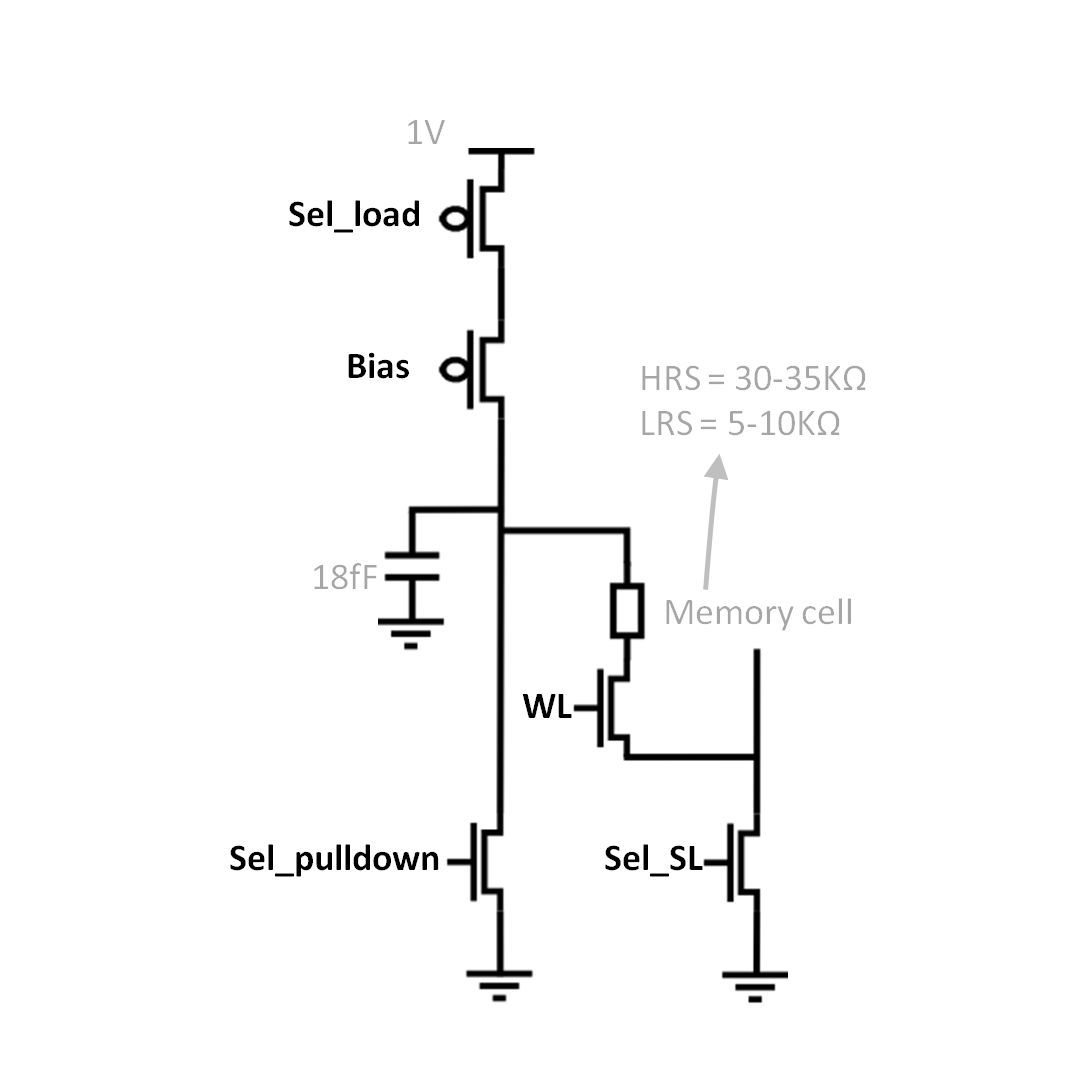
\includegraphics[width=0.45\textwidth] {../fig/hfdst-last-simsetup.png} \label{fig:simcircuit}}
\subfloat[Controle signalen 1]{ 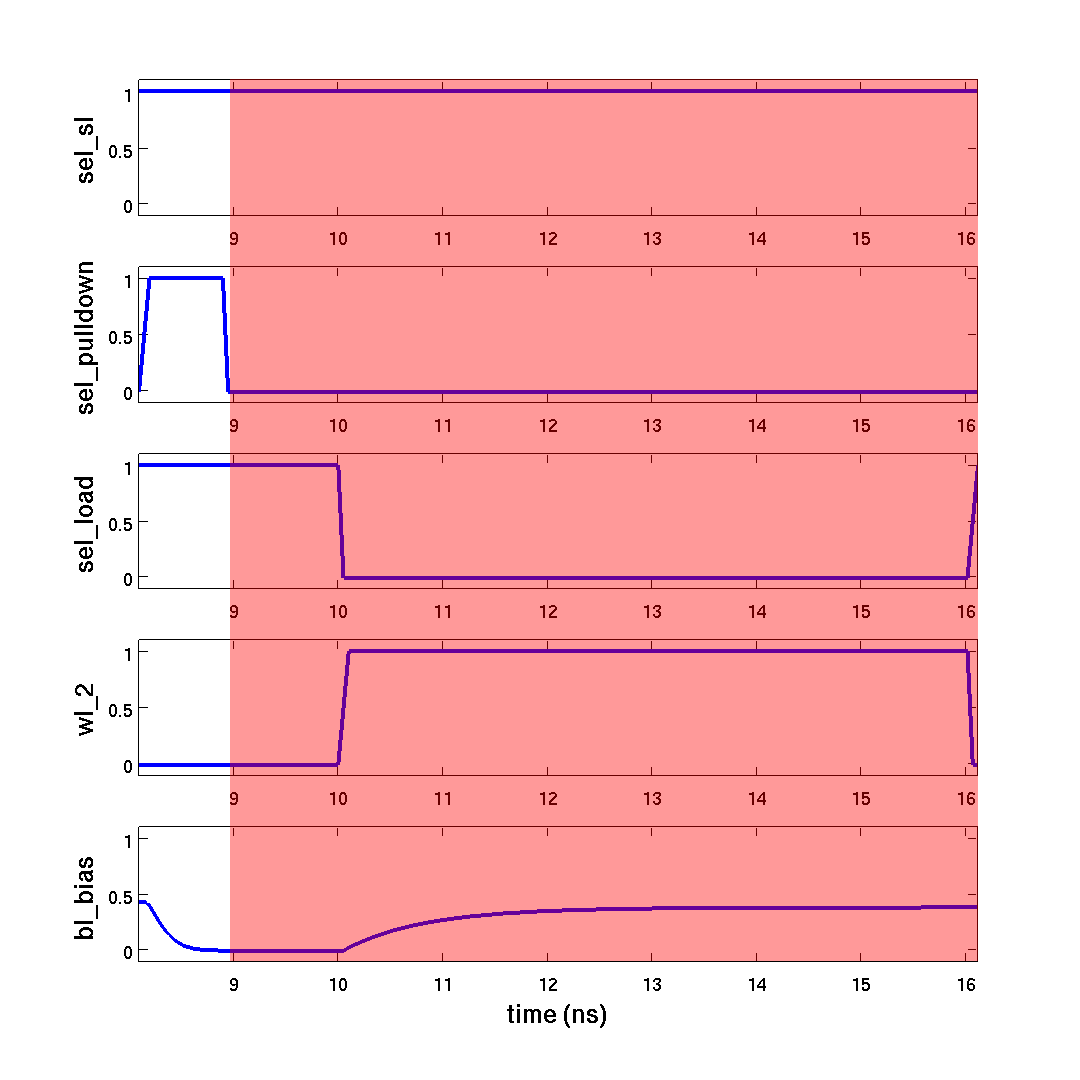
\includegraphics[width=0.45\textwidth] {../fig/hfdst-last-controlsig1.png} \label{fig:simcontr1}}\\
\subfloat[Controle signalen 2]{ 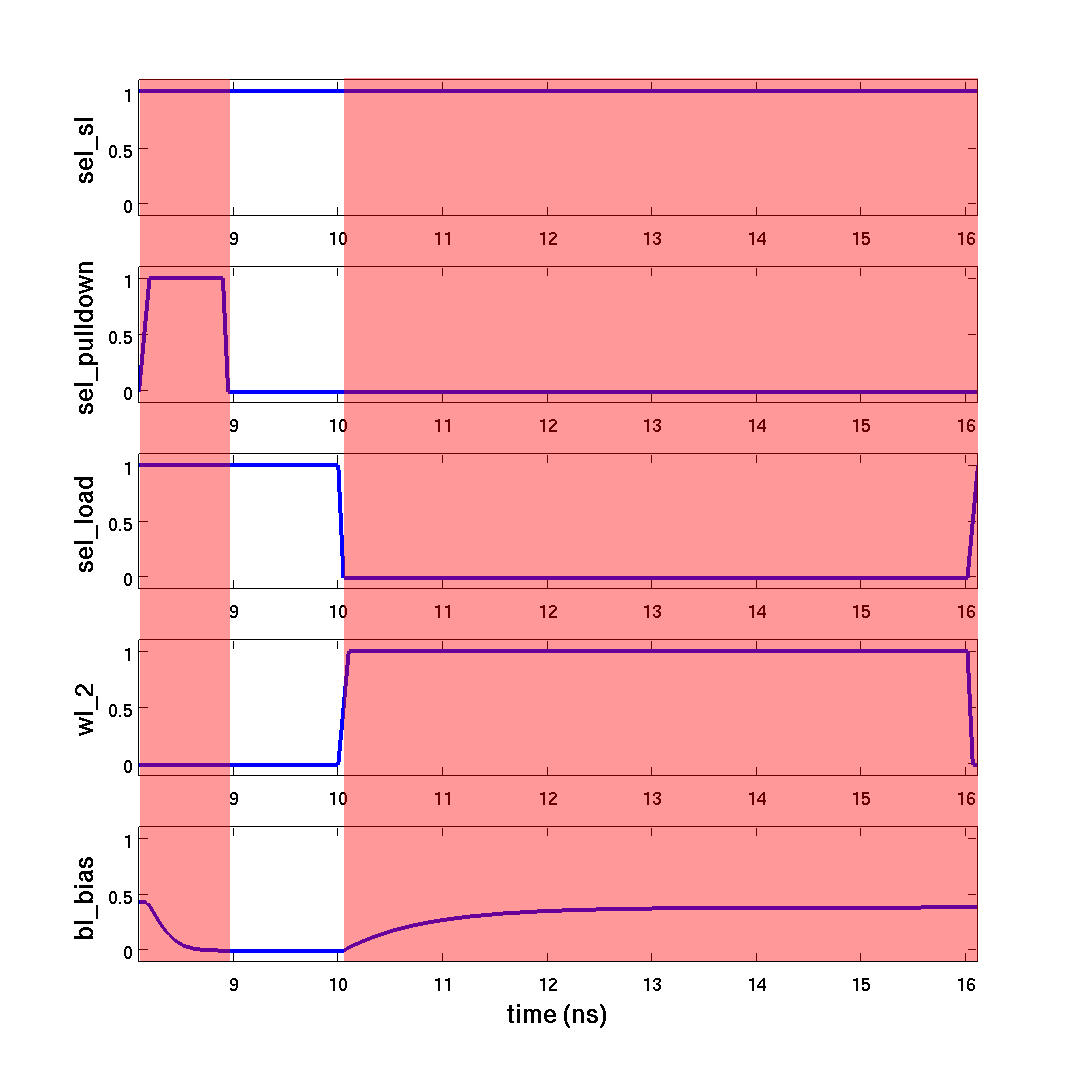
\includegraphics[width=0.45\textwidth] {../fig/hfdst-last-controlsig2.png} \label{fig:simcontr2}}
\subfloat[Controle signalen 3]{ 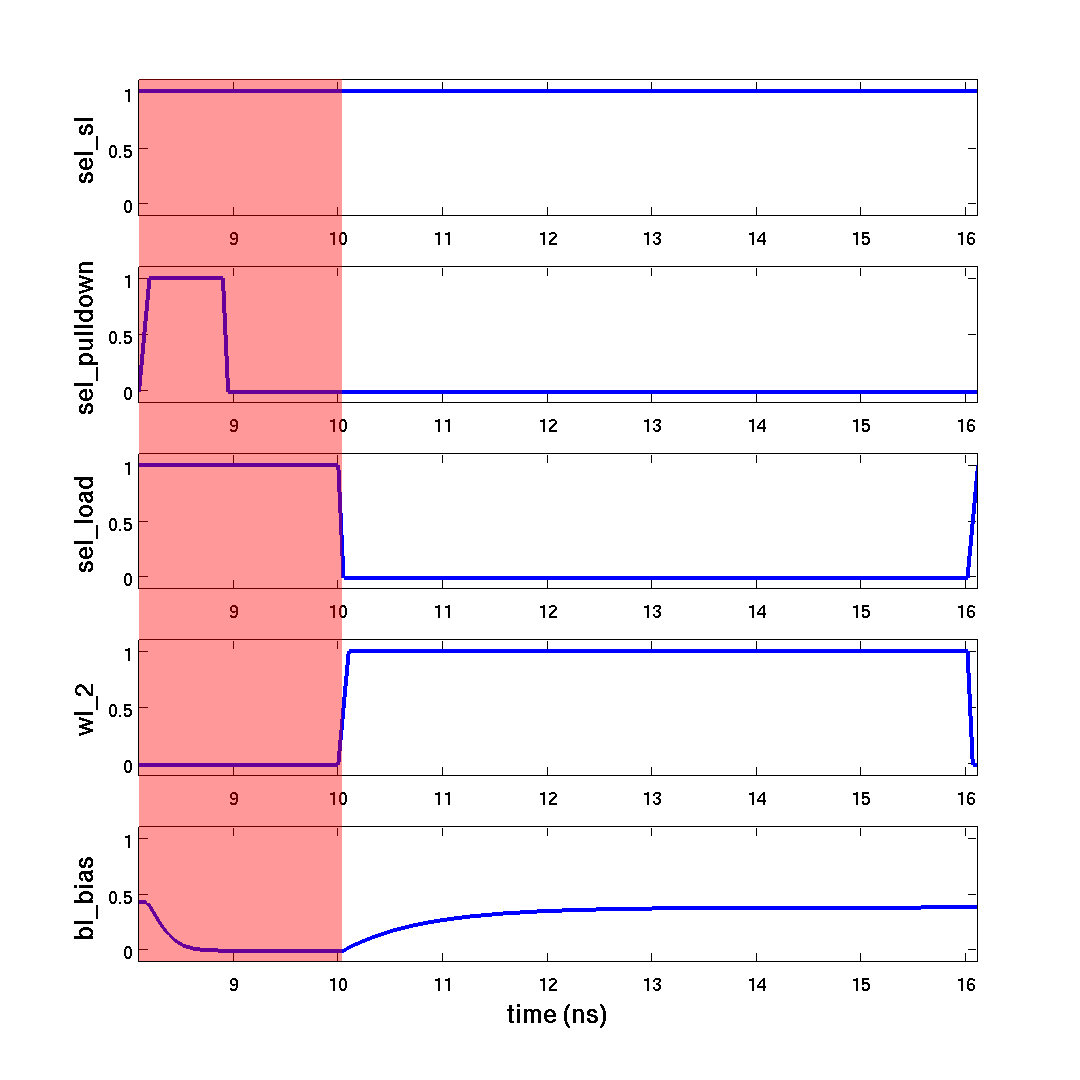
\includegraphics[width=0.45\textwidth] {../fig/hfdst-last-controlsig3.png} \label{fig:simcontr3}}
\caption{Test bench voor de last}\label{fig:simsetup}
\end{figure}

Eens een last gesimuleert is wordt het beoordeelt op het vlak van oppervlakte, bitlijn oplaadsnelheid, nominaal bitlijn voltage verschil en spanningsval over de cel. Het oppervlakte wordt berekend op basis van de lengtes en breetes van de last transistoren. De bitlijn oplaadsnelheid is de tijd dat nodig is om de bitlijn $99\%$ op te laden. Het nominale bitlijn voltageverschil is het verschil in bitlijnvoltage tussen een cell in HRS en LRS, wanneer de bitlijn $100\%$ opgeladen is. De bitlijn wordt veronderstelt $100\%$ opgeladen te zijn op het einde van de simulatie en de simulatietijd word voldoende lang gehouden om dit te garenderen. De spanningsval over de cell is belangrijk opdat de cell in van state wisselt gedurende de leescyclus. Aangezien de cell voorgesteld wordt met een weerstand zal dit natuurlijk nooit gebeuren maar dit is wel belangrijk moest er met echte memristors gewerkt worden. De numerieke waarde van de maximale spanningsval over de cel is heel erg afhankelijk van het type memristor. In dit onderzoek wordt er gewerkt met een maximum van 0.5V over de cell \cite{ppt:model}.

\section{vergelijking van verschillende types last}
Voor dit onderzoek worden vier mogelijke kandidaten van last vergeleken: de switchload (figuur \ref{fig:switchload}), de biasload (figuur \ref{fig:biasload}), de diodeload (figuur \ref{fig:diodeload}) en de bulkload (figuur \ref{fig:bulkload})\cite{bulkload}. Eerst wordt er een lineare sweep gedaan op de verschillende lasten (sectie \ref{sec:linload}), waarbij enkel de breetes en bias spanningen worden gesweept. De lengtes van de transistoren worden minimaal gehouden om er voor te zorgen dat de transistoren binnen de pitch van de bitlijn passen. Eens variabiliteit wordt toegevoegd aan de simulatie onder de vorm van monte-carlo (sectie \ref{sec:varload}), zal echter blijken dat er het verschil in bitlijnvoltage te klein is, en zal de lengte van de last transistoren ook moeten worden vergroot (sectie \ref{sec:finaleload}).

\begin{figure}[!ht]
  \centering
  \subfloat[De switch load]{\makebox[.22\textwidth]{ 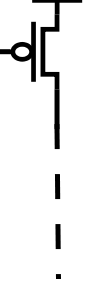
\includegraphics[width=0.12\textwidth] {../fig/hfdst-last-loadtypesswitch.png} \label{fig:switchload}}}
  \subfloat[De bias load]{\makebox[.22\textwidth]{ 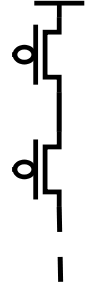
\includegraphics[width=0.12\textwidth] {../fig/hfdst-last-loadtypesbias.png} \label{fig:biasload}}}
  \subfloat[De diode load]{\makebox[.22\textwidth]{ 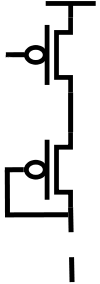
\includegraphics[width=0.12\textwidth] {../fig/hfdst-last-loadtypesdiode.png} \label{fig:diodeload}}}
  \subfloat[De bulk load]{\makebox[.22\textwidth]{ 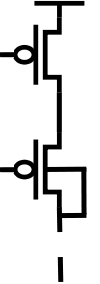
\includegraphics[width=0.12\textwidth] {../fig/hfdst-last-loadtypesbulk.png} \label{fig:bulkload}}}
  \caption{De verschillende types last}
  \label{fig:loads}
\end{figure}

\subsection{Lineaire sweep op de lasten}\label{sec:linload}
\paragraph{}
De switchload bestaat uit \'{e}\'{e}n pmos transistor die volledig wordt aan of afgesloten. Een lineare sweep met een breedte van de transistor tussen 100nm en 500nm werd gedaan en is geillustreed in figuur \ref{fig:switchloadsim}. Bij het vergroten van de breedte van de transistor zal de weerstand dalen en het verschil tussen de bitlijnen ook. Als we deze last vergelijken men het simpele model uit sectie \ref{sec:simplemodel}, zit de weerstand waarde aan de linker kant van de piek uit figuur \ref{fig:rpiek}. Bij het vergroten van de transistor breedte zal de bitlijn spanning stijgen en de spannings val over de cell dus ook. Verder volgt de risetime ook het simple model uit sectie \ref{sec:simplemodel}, waarbij de risetime daalt bij kleinere weerstandswaardes.

\paragraph{}
De biasload, is een last met twee pmos transistoren in serie. Bovenste van de twee wordt als een switch gebruikt en dus volledig aan of af gesloten. De onderste van de twee wordt op een spanning gebiased. Het voordeel van de biasload is dat men een grotere weerstand kan maken en dus de piek kan bereiken uit figuur \ref{fig:rpiek}. Dit kan men duidelijk zien op de x-assen van figuur \ref{fig:biasloadsim}. Ook hier zijn de breedtes van de transistoren gesweeepts tussen 100nm en 500nm. De bias spanning is tussen 0V en 0.4V gesweept. Een hogere bias spanning brengt echter geen nuttige bij drage. Door dat te kleinste weerstand dat met deze last te maken is ,binnen deze sweeprange, net iets groter is als deze van de switch load, is de biasload ook iets trager. De oplossingen waarbij dit het geval is, hebben echter een onbruikbaar verschill in bitlijn voltages. De spanningsval over de cell is vergeleken met de switch load heel wat hoger maar voor de meeste oplossingen ligt het nog altijd onder de limiet van 0.5V.

\paragraph{}
De diode load bestaat ook uit twee transistoren, de bovenste wordt net als bij de biasload als een switch gebruikt. De onderste is als een diode geconnecteerde transistor gekoppelt. Uit de sweept resultaten (figuur \ref{fig:diodeloadsim}) blijkt dat deze last heel snel is maar veel te kleinen bitlijn voltage verschillen heeft om bruikbaar te zijn.

\paragraph{}
De bulkload werd voorgestelt in de paper van Ren et al. \cite{bulkload} als een goede kandidaat omwille van zijn grote uitgangsimpedantie. Deze last bestaat uit een switch transistor en een bulk geconnecteerde transistor. Deze bulk geconnecteerde transistor wordt op 0V gebiast aangezien deze de beste resultaten gaf. De breedtes van de transistoren zijn gesweept tussen 100nm en 500nm. De resultaten van deze sweep zijn geillustreerd in figuur \ref{fig:bulkloadsim}. In de resultaten kan gezien worden dat deze last zich vergelijkbaar gedraagt als de biaslast. Enkel op het vlak van risetime zijn er oplossingen die beter zijn.

\afterpage{
\begin{figure}
  \centering
  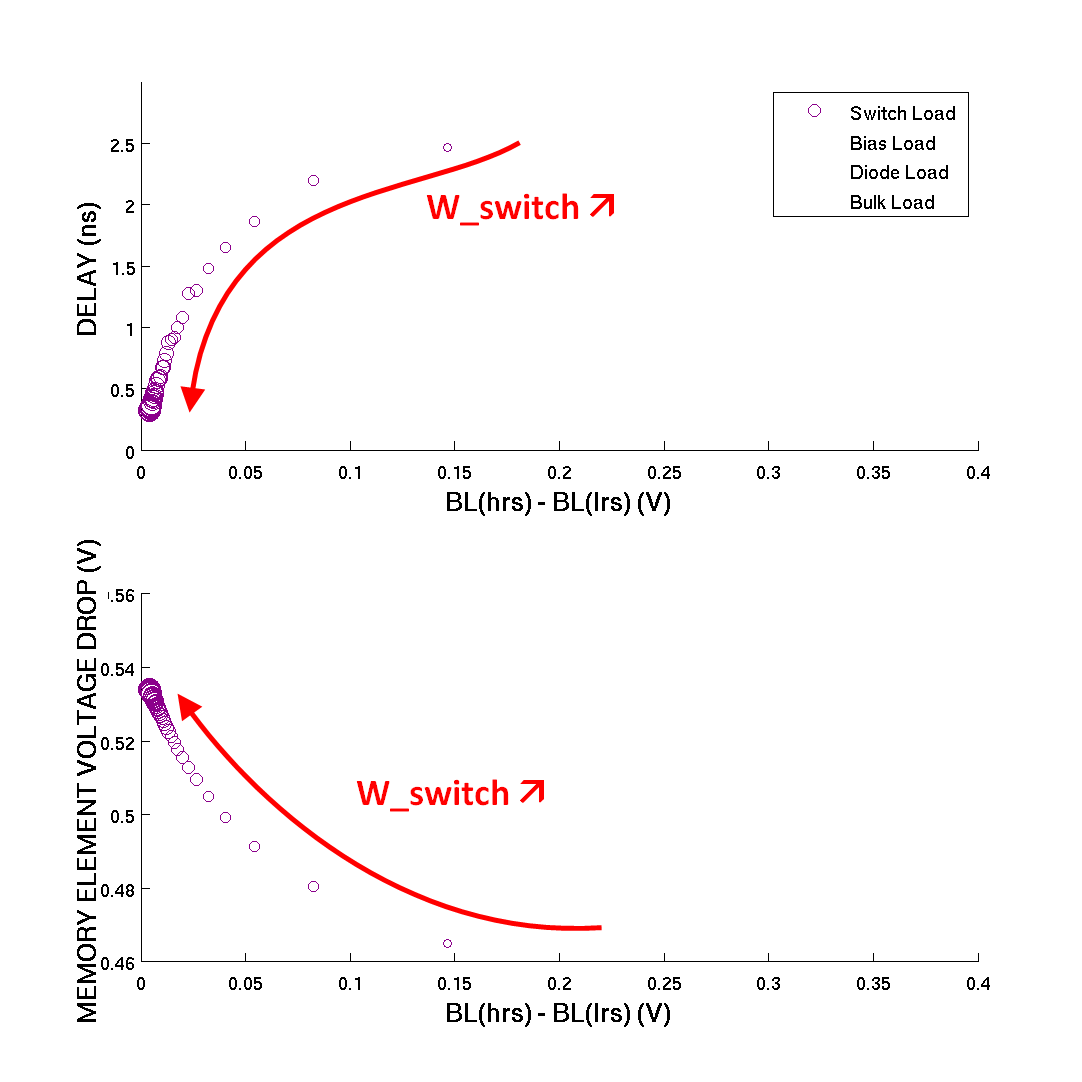
\includegraphics[width=0.67\textwidth]{../fig/hfdst-last-switchload.png}
  \caption{Lineaire sweep van switchload}
  \label{fig:switchloadsim}
 \centering
  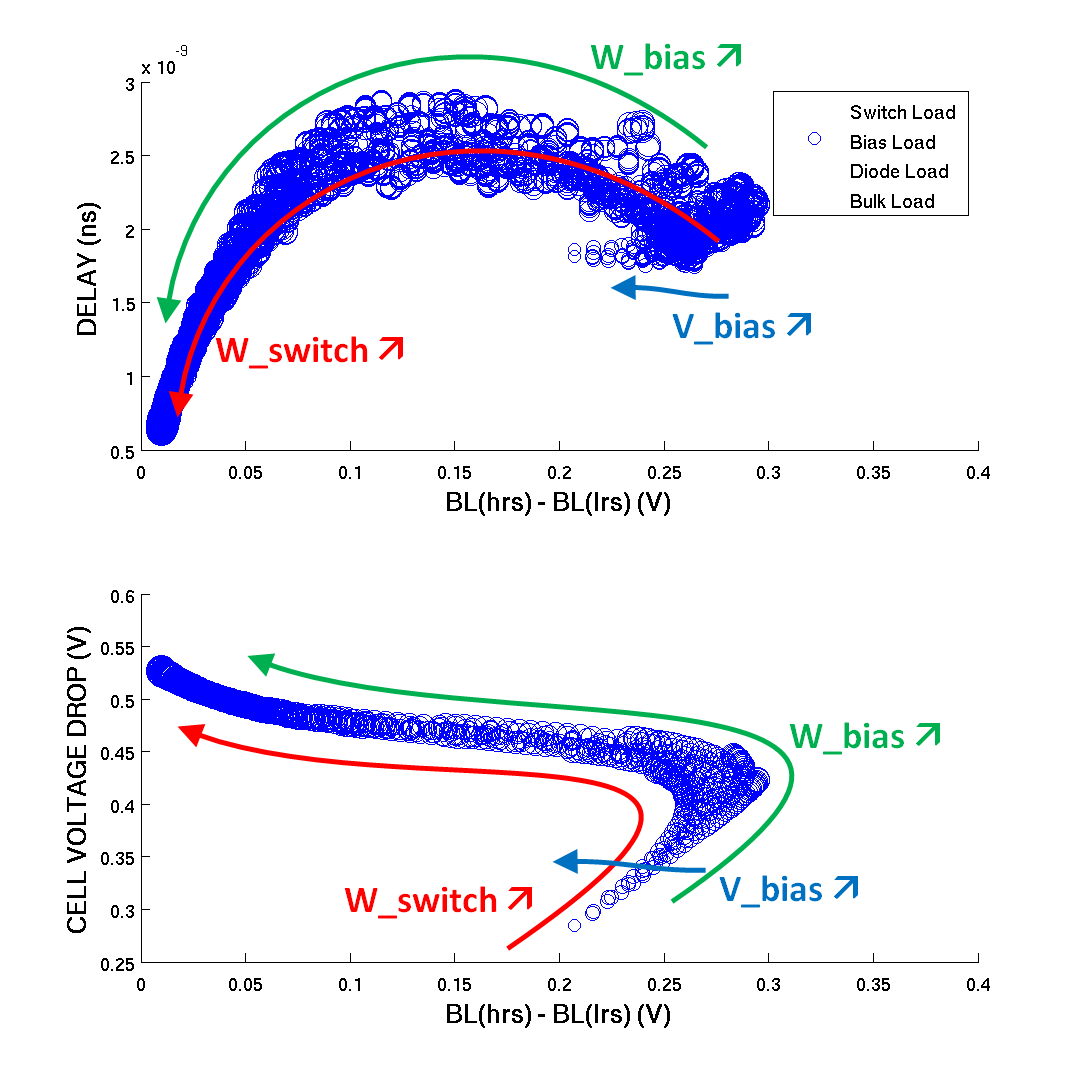
\includegraphics[width=0.67\textwidth]{../fig/hfdst-last-biasload.png}
  \caption{Lineaire sweep van biasload}
  \label{fig:biasloadsim}
\end{figure}
}
\afterpage{
\begin{figure}
  \centering
  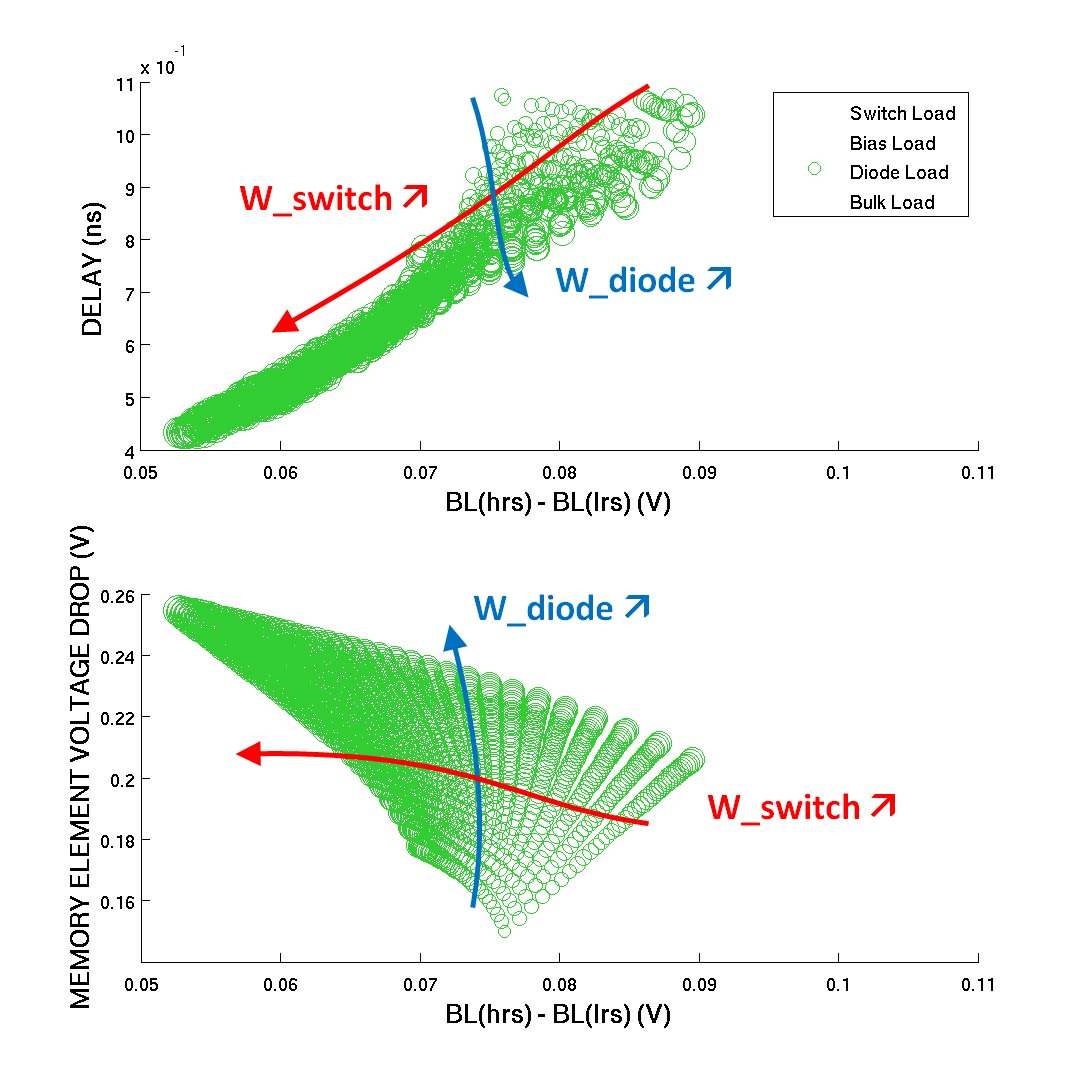
\includegraphics[width=0.67\textwidth]{../fig/hfdst-last-diodeload.png}
  \caption{Lineaire sweep van diodeload}
  \label{fig:diodeloadsim}
  \centering
  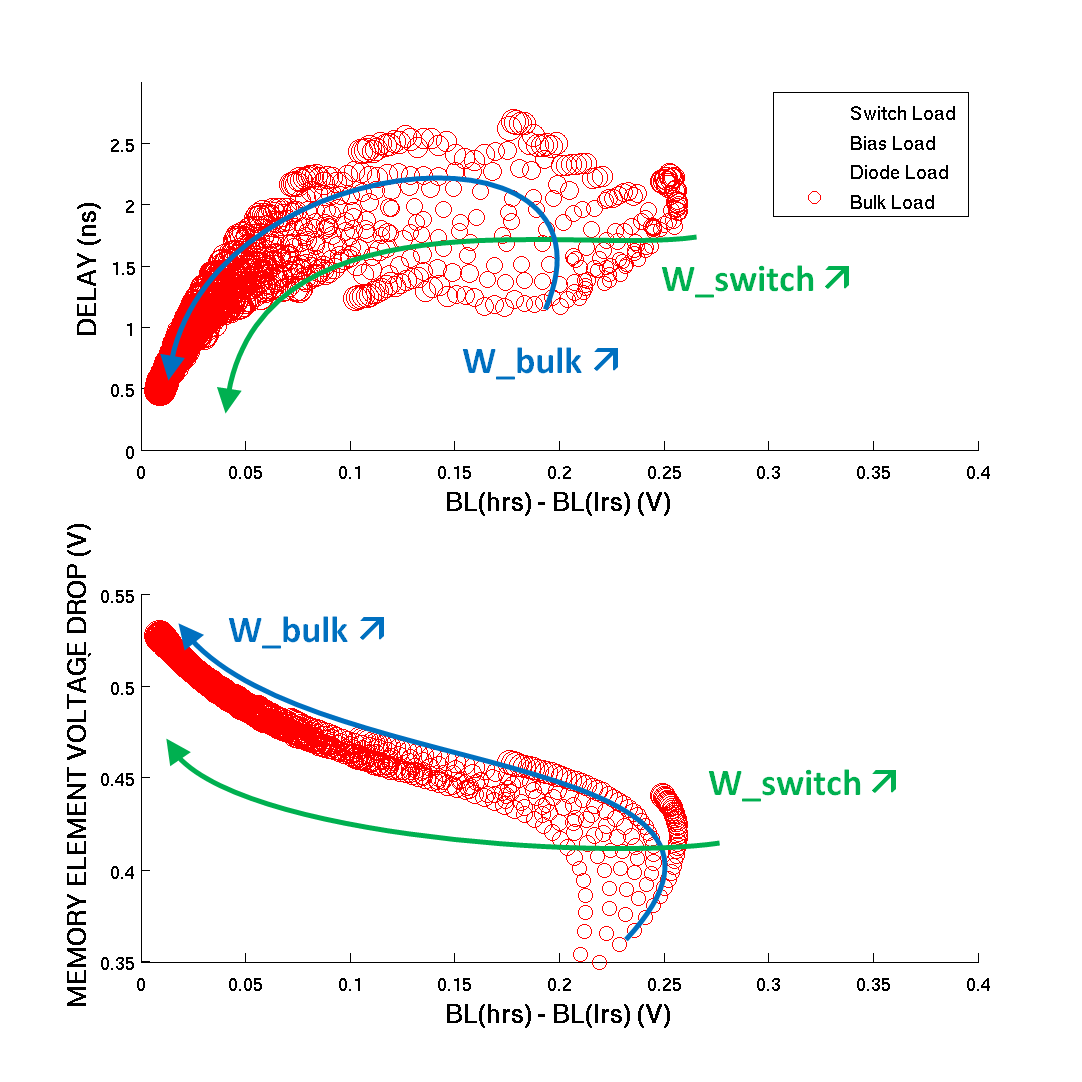
\includegraphics[width=0.67\textwidth]{../fig/hfdst-last-bulkload.png}
  \caption{Lineaire sweep van bulkload}
  \label{fig:bulkloadsim}
\end{figure}
}

\subsection{Het toevoegen van variabiliteit}\label{sec:varload}
Na een selectie te hebben gemaakt van de oplossingen uit de vorige sectie, worden met deze oplossingen nieuwe simulaties gedaan waarbij er variabiliteit is toegevoegt. Deze variabiliteit is toegevoegd op alle transistoren in het test circuit en op de weerstands waarde van de geheugen cellen. Voor de transistoren word er een Pelgrom constante voor vt van $2.5mV\mu m$ gebruikt en voor $\beta$ van $1.2\mu m$ gebruikt \cite{ppt:variatie}. Voor de weerstandswaarde van de memristors wordt er een gausische verdeling gebruikt met nominale waardes 7.5k$\Omega$ en 32.5k$\Omega$ en met $\sigma = 0.833k\Omega$. Er worden telkens 500 monte carlo simulaties gedaan per oplossing. Hierna worden de bitlijn voltages van cellen met een HRS en LRS gefit op een gausische distributie. De oplossing met het grootste bitlijn voltage verschil tussen de extrema van HRS en LRS is een biasload met een switch transitor breete van 100nm, een bias transistor breete van 180nm en een bias voltage van 0V. De bitlijn spanning distributies zijn geillustreed op figuur \ref{fig:distbias}. Het voltage verschill tussen de CDF = $0.1\%$ van HRS en CDF = $99.9\%$ van de LRS is 65mV. Dit is niet veel aangezien de distributie van het bitlijn voltage van de referentie cell hier tussen moet passen en er daarna nog marge over moet zijn voor variabiliteit in de senseamplifier. De invloed van de variabiliteit op de transistoren in de last is even groot voor beide transisoren.

\begin{figure}[!ht]
  \centering
  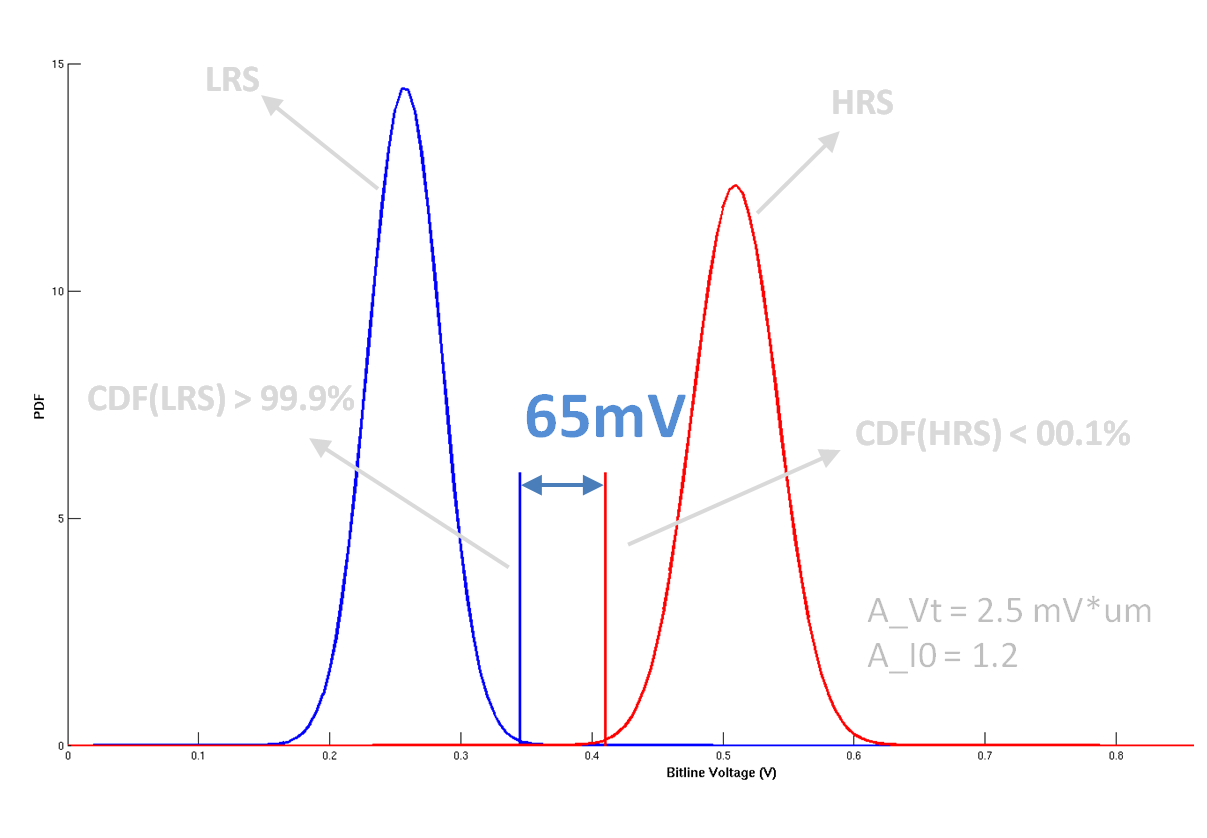
\includegraphics[width=0.67\textwidth]{../fig/hfdst-last-var1.png}
  \caption{Bitlijn voltage distributie voor een biasload}
  \label{fig:distbias}
\end{figure}

Figuur \ref{fig:distref} stelt de distributie van de bitlijn spanning van de referentie cellen voor. Hierbij varieert het aantal referentie cellen van 2 tot 30 en er werd een even groot aantal referentie cell in HRS als LRS gehouden. Zoals gezien kan worden, heeft men een heel aantal cellen nodig heeft om een distributie breete van 39mV te krijgen. Dit geeft dan een marge van ongeveer 10mV voor de senseamplifier, indien de voorgaande vermedelde biasload gebruikt wordt, wat helemaal niet veel is. Daarom wordt de constraint waarbij de transistor lengte minimaal gehouden wordt opgeheven in de volgende sectie.

\begin{figure}[!ht]
  \centering
  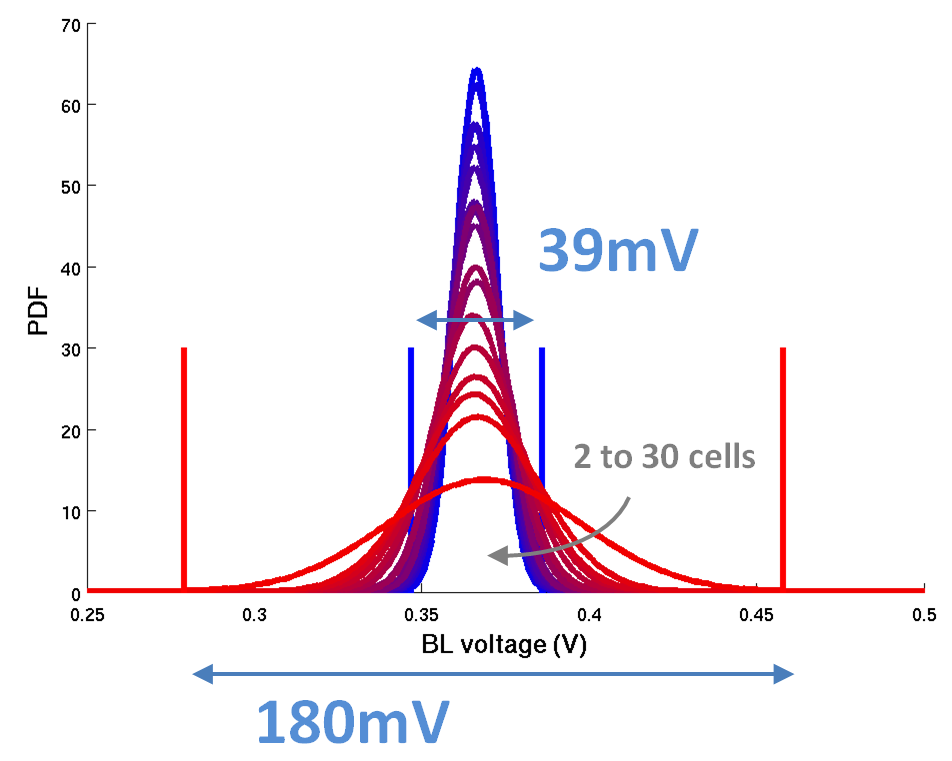
\includegraphics[width=0.67\textwidth]{../fig/hfdst-last-ref.png}
  \caption{Lineaire sweep van switchload}
  \label{fig:distref}
\end{figure}


\subsection{De transistor lengte vergroten}\label{sec:finaleload}
Om de variabiliteit onder controle te houden moeten de transistoren vergroot worden. Twee opties worden hiervoor overwogen. De eerste is het toevoegen van een derde transistor in serie. Om dezelfde lastimpedantie te bekomen als voor 2 transisoren in serie, moeten alle drie transistoren een grote breete hebben wat zou betekenen dat ze groter zijn en minder gevoelig voor mismatch. Een aspect waar geen rekening mee wordt gehouden in die redenering is de toestand waarin deze transistoren zich bevinden. Bij drie transistoren in serie zal de onderste van de drie zich in near- tot sub-theashold bevinden. De stroom in het sub-theshold gebied is exponentieel met de gate-source spanning dit levert een grote variatie in de stroom voor kleine vt mismatch. Dit fenemeen zien men niet bij 2 transistoren in serie, aangezien de transistoren hier in het lineare gebied zijn. Daarom wordt er gekozen voor een tweede optie om de mismatch onder controle te houden namelijk het vergroten van de lengte van de transistor. Als men de lengte vergroot, Stijgt de weerstand wat dan weer gecompenseert kan worden door de breedte ook wat te vergroten. Nu men deze constraint laten varen heeft, wordt er dan ook geopteert om een switchload ipv een bias load te gebruiken, omwille van zijn simpliciteit.\\
Figuur \ref{fig:length} geeft de resultaten weer van een sweep van verschillende lengtes en breetes voor een switchload. De resultaten worden voorgestelt in functie van $W/L$ wat een indicatie is voor de weerstand van de transistor. In de bovenste figuur kan men duidelijk een maximun zien voor het verschil in bitlijn voltage zoals in sectie \ref{sec:simplemodel} werd voorspelt. Verder wordt opgemerkt dat er best \'{e}\'{e}n van de oplossingen aan de linkerkant van het maximum gekozen wordt aangezien de spanningsval over de cel van de oplossingen aan de rechterkant van het maximum te hoog zijn.
\begin{figure}[!ht]
  \centering
  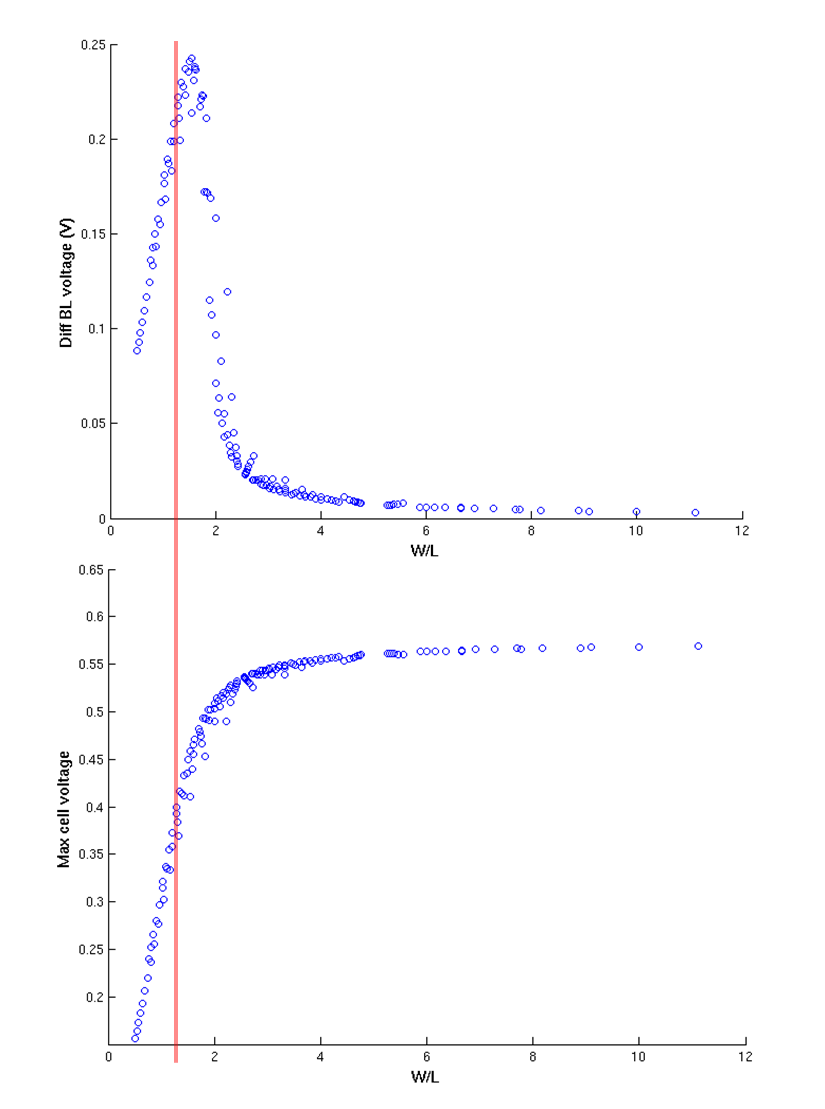
\includegraphics[width=0.66\textwidth]{../fig/hfdst-last-length.png}
  \caption{Verschillende oplossingen voor de switchload met variabele lengtes en breetes}
  \label{fig:length}
\end{figure}

Voor de finale last wordt er geopteert voor een transistor met lengte gelijk aan 198nm en breedte gelijk aan 300nm. Op figuur \ref{fig:length} word deze aangeduid met de rode lijn. Op figuur \ref{fig:distswitch} wordt de bitlijn spanning distributie van deze last getoont. Het minimale verschil in bitlijn spanning is bijna 200mV. De distributie van bitlijn voltage van de referentie is ook aangegeven op deze figuur. Deze bestaat hier uit 4 referentie cellen waarvan 2 in HRS en 2 in LRS. Opvallend is dat deze referentie niet in het centrum zit tussen de bitlijn voltages van de cellen. Dit kan opgelost worden door een niet gelijk aantal referentie cellen in HRS en LRS te hebben. Aangezien de standaarddeviatie op de bitlijn voltages heel wat beter is, nu de lengte van de transistoren ook wordt gesized, kan er gerust gekozen worden voor een last met een kleiner nominaal verschil in bitlijn voltages \label{anderelast}. Dit kan 2 voordelen met zich mee brengen. Het eerste is dat de spanningsval over de cel verlaagt kan worden als met voor een oplossing kiest dan links zit van het maximum in figuur \ref{fig:length}. Het tweede voordeel is dat men voor een oplossing kan kiezen waarbij de bitlijn voltages lager zijn wat een energie winst kan opleveren. Ondanks deze voordelen werd er toch geopteert voor de oplossing met het grootste bitlijn voltage verschil.

\begin{figure}[!ht]
  \centering
  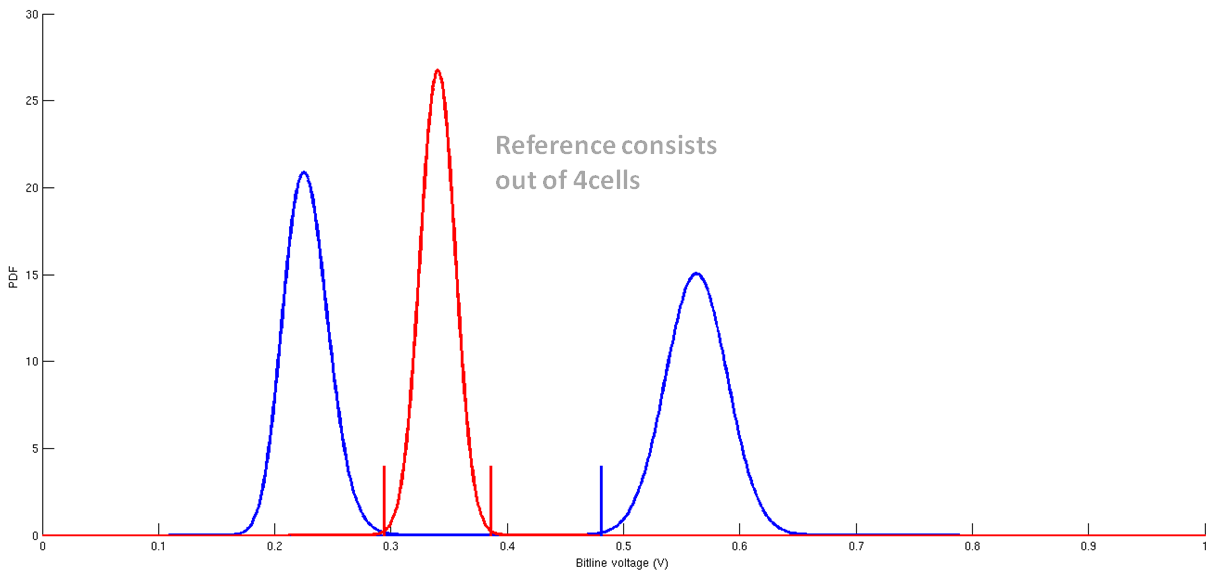
\includegraphics[width=0.67\textwidth]{../fig/hfdst-last-var2.png}
  \caption{Bitlijn voltage distributie voor de finale load}
  \label{fig:distswitch}
\end{figure}

\section{Besluit}
Verschillende kandidaten voor lastimpedanties werden overwogen. Aanvankelijk werd er getracht een last met minimale transistorlengtes te vinden, dit bleek echter niet haalbaar wanneer variabiliteit in rekening wordt genomen. Een enkele transitor met niet-minimale afmetingen bleek de beste resultaten te leveren wat betreft BL-spanningsverschil en spanningsval over geheugenelement.
\chapter{Sense Amplifier analyse}
\label{sensamp}
Een sense amplifier versterkt kleine signaalverschillen tot rail-tot-rail signalen. Aangezien de uitgangsignalen hiervan ook de uitgelezen bits zijn van het geheugen, is het bovenal belangrijk dat dit op een correcte manier gebeurt, ondanks variabiliteit.
Het is dus logisch om de sense amplifier wat meer te onderzoeken en zodanig te ontwerpen op een robuuste manier, terwijl er ook rekening gehouden wordt met energie en snelheid.

\section{Types SA}
...
\begin{figure}
  \centering
  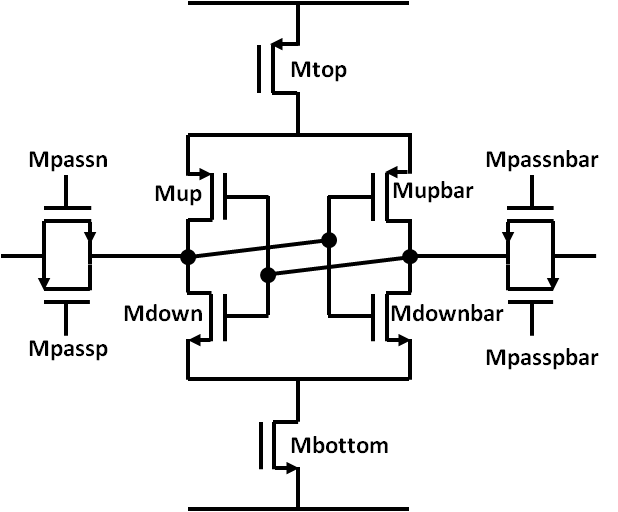
\includegraphics[scale=0.4]{../fig/hfdstk-sensamp-ourSA.png}
  \caption{een sense amplifier}
  \label{fig:ourSA}
\end{figure}

In wat volgt zal er worden voortgewerkt met de SA van figuur \ref{fig:ourSA}.


\section{Offsetspanning}
Een ideale sense amplifier zal voor elke twee ingangssignalen correct versterken, tenzij de signalen dezelfde zijn, waarna de SA in een metastabiele toestand belandt. In de praktijk is er echter wegens variabiliteit een limiet voor het ingangsspanningsverschil waarbij er correct versterkt wordt. Deze limiet heet de offsetspanning en wordt geïllustreerd in figuur \ref{fig:offset}. De offsetspanning van een SA is in de ontwerpfase een stochastische variabele met gemiddelde 0V, pas nadat een chip gefabriceerd is ligt de offsetspanning definitief vast [al kan het zijn dat deze met de tijd nog verandert].
Er zijn 2 manieren waarop men de offsetspanning van een systeem kan aanpakken: ofwel ontwerp je het systeem zodanig dat het verschil van de ingangssignalen van de SA groot genoeg is zodat ze [in 99,9\% van de gevallen] niet groter is dan de offsetspanning, ofwel bouw je een mechanisme in waarbij je na fabricatie de offsetspanning meet en vervolgens compenseert. In dit werk is gekozen voor het eerste.
Hiervoor is het wel belangrijk te onderzoeken wat de verdeling is van de offsetspanning, dit wordt gedaan in de volgende sectie.

\begin{figure}
  \centering
  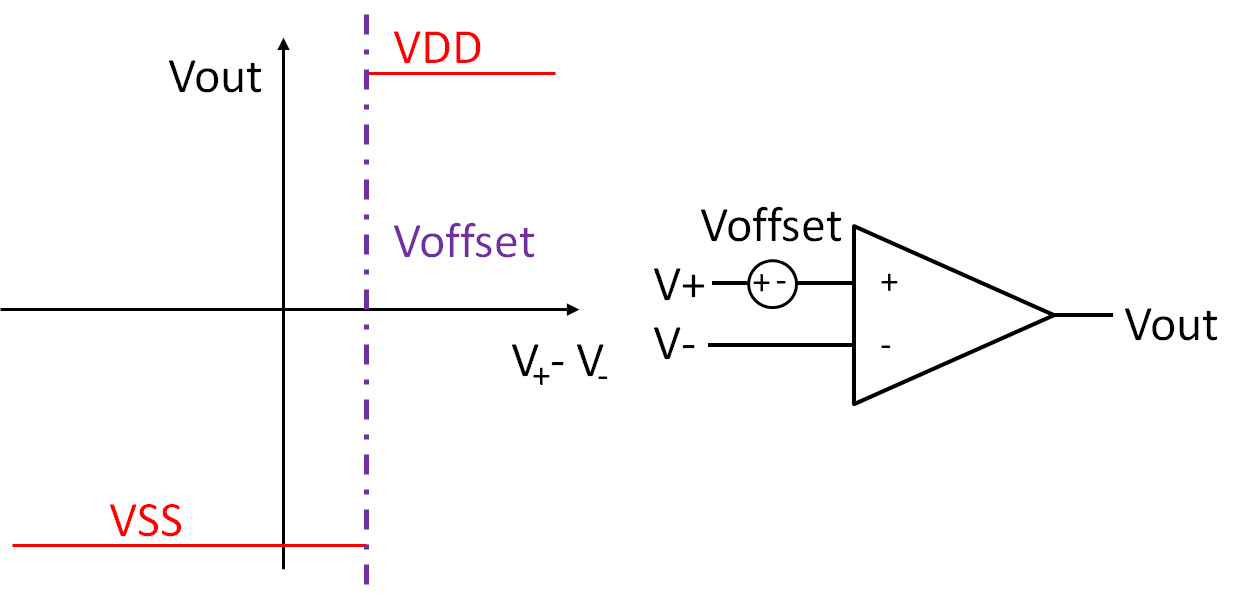
\includegraphics[scale=0.4]{../fig/hfdstk-sensamp-offset.png}
  \caption{Illustratie van offsetspanning}
  \label{fig:offset}
\end{figure}

\section{Sensitiviteitsanalyse}
De SA wordt gerealiseerd als een circuit met transistors. Elke transistor heeft 2 stochastische parameters met een normale verdeling, nl. $\Delta V\textsubscript{t}$ en $\Delta \beta$. De spreiding van deze verdelingen is gekend: $\sigma_{\Delta V_{t}} = \frac{A\textsubscript{V\textsubscript{t}}}{\sqrt{W L}}$ en $\sigma_\frac{{\Delta \beta}}{\beta} = \frac{A_{\beta}}{\sqrt{W L}}$. Met een sensitiveitsanalyse kan men uit deze standaardafwijkingen de standaardafwijking van de offsetspanning $\sigma_{V_{offset}}$ berekenen. Hierbij wordt verondersteld dat de stochastische variabele $V_{offset}$ een lineaire combinatie is van de normaal verdeelde afwijkingen $(\Delta V_{t})_{i}$ en $(\frac{\Delta_{\beta}}{\beta})_{i}$: $V_{offset}=\sum\limits_{i=1}^{N} a_{i} (\Delta V_{t})_{i} + b_{i} (\frac{\Delta_{\beta}}{\beta})_{i}$.
$a_{i}$ en $b_{i}$ zijn de gevoeligheden van de offset naar de variatieparameters: $a_{i}=\frac{\partial V_{offset}}{\partial (\Delta V_{t})_{i}}$ en $b_{i}=\frac{\partial V_{offset}}{\partial (\frac{\Delta_{\beta}}{\beta})_{i}}$.
Voor een dergelijke variabele geldt dan: $\sigma_{V_{offset}}=\sqrt{\sum\limits_{i=1}^{N} a_{i}^{2} (\sigma_{\Delta V_{t}})_{i}^{2} + b_{i}^{2} (\sigma_{\frac{\Delta_{\beta}}{\beta}})_{i}^{2}}$.

Er moet wel geverifieerd worden of de stelling dat er een lineaire afhankelijkheid is tussen $V_{offset}$ en de variatieparameters gegrond is.
Dit kan gedaan worden aan de hand van een analyse waarbij elke variatieparameter afzonderlijk gesweept wordt. 

\subsection{Sensitiviteitsanalyse op een minimale SA}
In figuur \ref{fig:min-sensanalysis} wordt het resultaat getoond voor een dergelijke analyse bij een SA met minimale afmetingen, in tabel \ref{tab:min-sensanalysis} worden de resultaten en de resulterende standaardvariatie van de SA getoond.
Er moet opgemerkt worden dat er bij deze simulatie slechts gesweept werd voor de variatieparameters van -4$\sigma$ tot 4 $\sigma$. Dit is om de reden dat voor de minimale transistoren de standaardvariatie het grootst is. In de Spectre-simulaties zouden transistoren voor te grote negatieve $\beta$-mismatch stroom leveren in de omgekeerde richting. Deze situatie zal fysisch nooit optreden.

\begin{table}
\begin{tabular}{|c|c|c|c|c|c|}
\hline Transistor & Parameter & Richtingscoëfficiënt [$\frac{mV}{\sigma}$] & W [nm] & L [nm] & $\sigma$ \\ 
\hline Mupbar & Vt & 22.733 & 100 & 45 & 37.2678mV \\ 
\hline Mup & Vt & -22.250 & 100 & 45 & 37.2678mV \\ 
\hline Mupbar & $\beta$ & 13.583 & 100 & 45 & 17.8885\% \\ 
\hline Mpassn & $\beta$ & 13.467 & 100 & 45 & 29.8142\% \\ 
\hline Mpassbarn & $\beta$ & -13.117 & 100 & 45 & 29.8142\% \\ 
\hline Mup & $\beta$ & -13.033 & 100 & 45 & 17.8885\% \\ 
\hline Mdownbar & $\beta$ & -9.383 & 100 & 45 & 29.8142\% \\ 
\hline Mdown & Vt & -9.267 & 100 & 45 & 42.0381mV \\ 
\hline Mdownbar & Vt & 9.233 & 100 & 45 & 42.0381mV \\ 
\hline Mdown & $\beta$ & 8.217 & 100 & 45 & 29.8142\% \\ 
\hline Mpassp & $\beta$ & -4.50 & 100 & 45 & 17.8885\% \\ 
\hline Mpassbarp & $\beta$ & 4.383 & 100 & 45 & 17.8885\% \\ 
\hline Mpassbarp & Vt & 0.70 & 100 & 45 & 37.2678mV \\ 
\hline Mpassp & Vt & -0.70 & 100 & 45 & 37.2678mV \\ 
\hline Mbottom & $\beta$ & 0.083 & 100 & 45 & 29.8142\% \\ 
\hline Mbottom & Vt & -0.033 & 100 & 45 & 42.0381mV \\ 
\hline Mpassbarn & Vt & 0 & 100 & 45 & 42.0381mV \\
\hline Mpassn & Vt & 0 & 100 & 45 & 42.0381mV \\
\hline Mtop & Vt & 0 & 100 & 45 & 37.2678mV \\
\hline Mtop & $\beta$ & 0 & 100 & 45 & 17.8885\% \\
\hline 
\hline & $\sigma_{Voffset}$: & 45.6813mV & & & \\
\hline
\end{tabular} 
\caption{Sensitiviteitsanalyse van de minimale SA}
\label{tab:min-sensanalysis}
\end{table}

Opmerkelijk bij deze analyse is dat er een significante bijdrage is van de pass-gates door $\beta$-mismatch. Een nadere observatie leert dat deze bijdrage optreedt door ladingsinjectie van de pass-gates die niet meer gematched is (zie figuur \ref{fig:chargeinjectionmismatch}).
Hierbij moet wel worden opgemerkt dat voor deze simulatie er geen overlap is tussen het controlesignaal op de passgate aan te zetten en het signaal om de SA te activeren.
De reden hierachter is dat als er overlap tussen deze signalen is, de SA ook de BL zou trachten op te laden. Hierbij zou er moeten ingeboet worden aan snelheid en het zou ook extra energie kosten.

Men kan argumenteren dat er een korte overlap zou kunnen toegelaten zijn, waarna er voldoende spanningsverschil tussen de 2 ingangs-uitgangsknopen zou opgebouwd zijn opdat de ladingsinjectie geen effect meer kan hebben op het eindresultaat. Een tegenargument is dat de timing hiervoor te precies moet zijn.
\begin{figure}
  \centering
  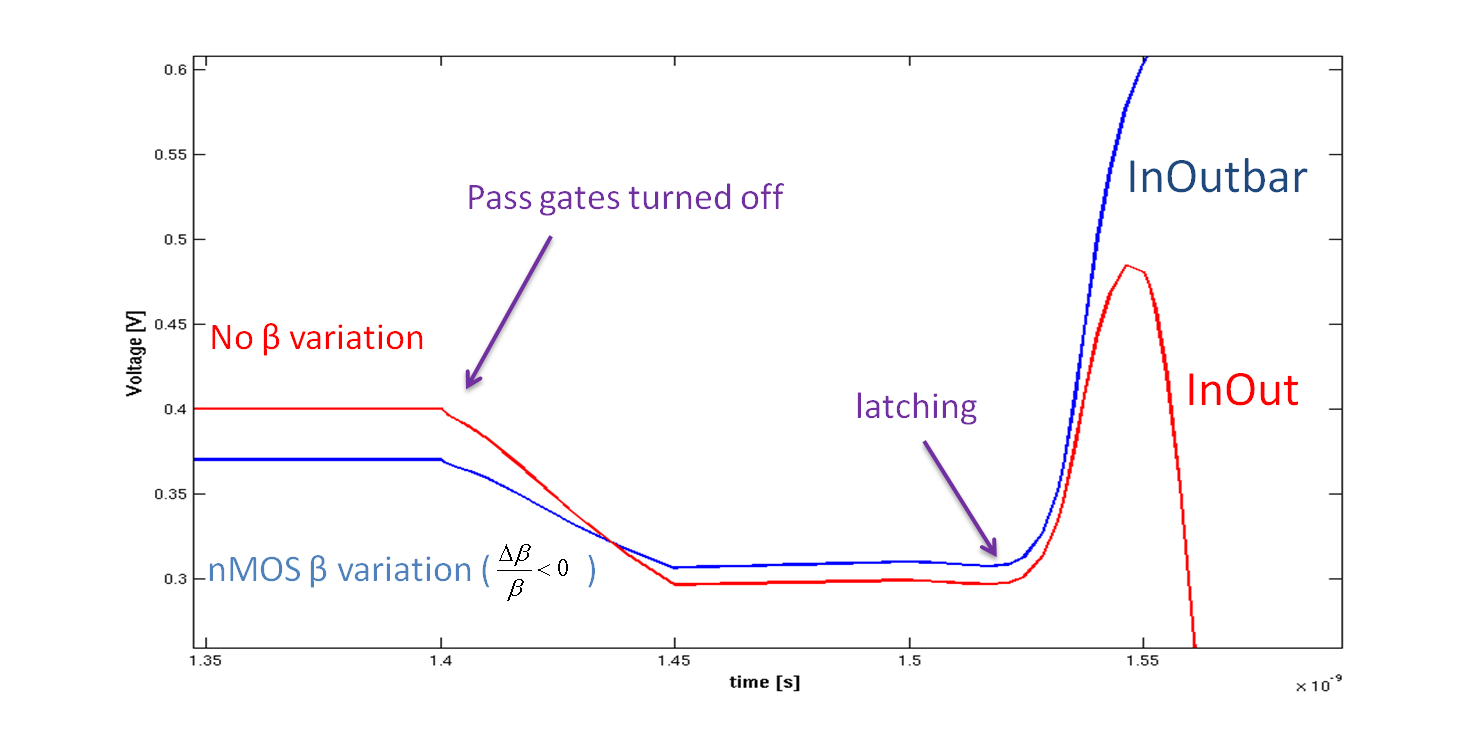
\includegraphics[scale=0.4]{../fig/hfdstk-sensamp-chargeinjectionmismatch.png}
  \caption{Door $\beta$-mismatch is ladingsinjectie van de pass-gates niet meer gematched en gaat de SA foutief latchen}
  \label{fig:chargeinjectionmismatch}
\end{figure}

\subsection{RC-latch-effect}
\label{RC-latch-effect}
De situatie waarbij er volledige overlap is tussen de controle signalen kan vereenvoudigd worden opgesteld met de situatie van figuur \ref{fig:RC-latch}. De pass-gate die aanstaat wordt voorgesteld als een weerstand, de pass-gate in het local block en diens parasitaire capaciteit wordt verwaarloosd. CL bedraagt voor deze simulatie 46 fF, het equivalent voor een BL waaraan 256 cellen hangen. Cint bedraagt voor een SA met minimale transistorafmetingen 161 aF. Wanneer het dynamisch latch-gedrag bekeken wordt voor verschillende waardes van R, treedt er een merkwaardig effect op (zie figuur \ref{fig:RC-latch-sim}): voor voldoende grote waardes van R lijkt het alsof de grote capaciteit ontkoppeld is van de latch tot op een zeker tijdstip, waarna een veel tragere settling optreedt.
\begin{figure}
  \centering
  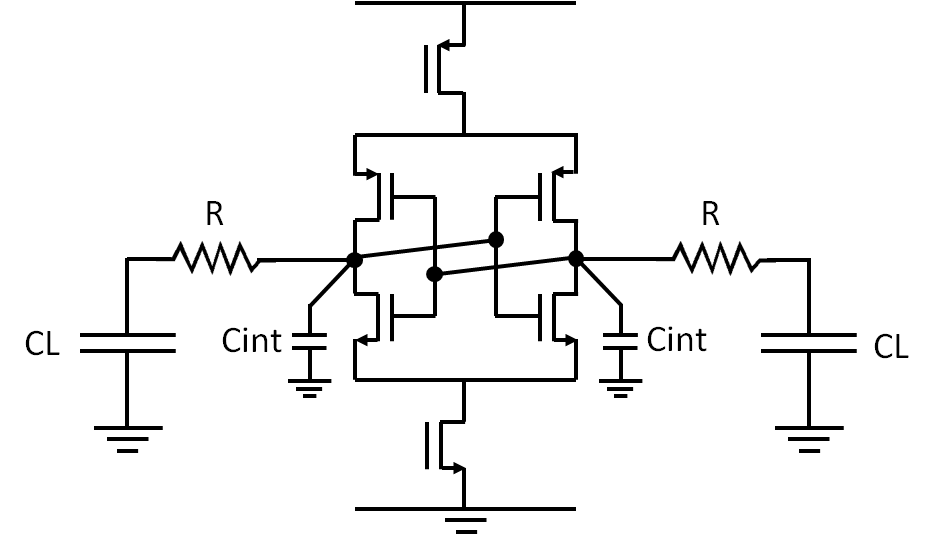
\includegraphics[scale=0.4]{../fig/hfdstk-sensamp-RC-latch.png}
  \caption{Simulatieopstelling voor het RC-latch-effect}
  \label{fig:RC-latch}
\end{figure}
\begin{figure}
  \centering
  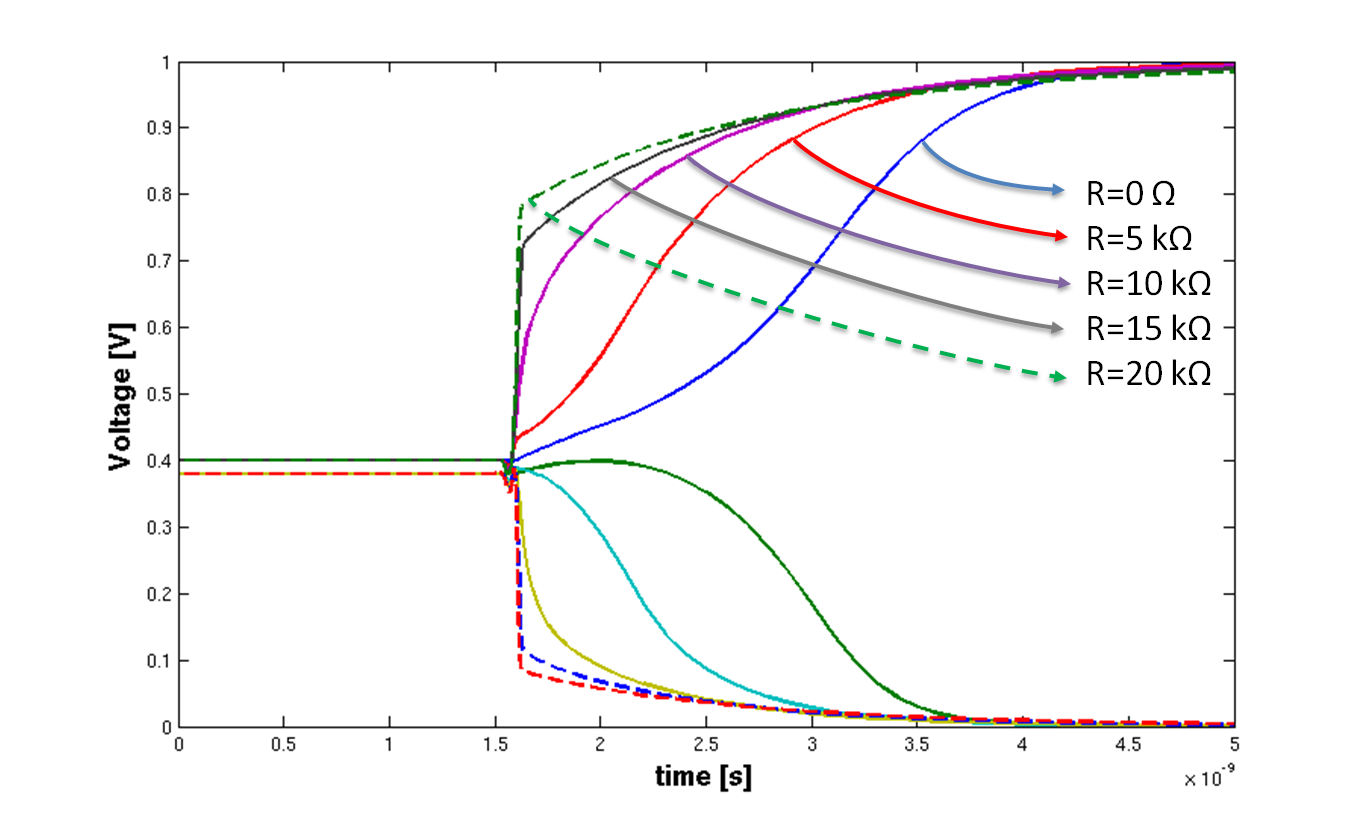
\includegraphics[scale=0.4]{../fig/hfdstk-sensamp-RC-latch-sim.png}
  \caption{Simulatieresultaten voor het RC-latch-effect:de 2 ingangs-uitgangsknopen zijn voorgeladen op 400mV en 380mV. Na 1,6ns wordt de SA aangezet. De SA is ideaal voor deze simulatie.}
  \label{fig:RC-latch-sim}
\end{figure}
De verklaring ligt in het feit dat CL zich voor hoge frequenties als een kortsluiting gedraagt (zie figuur \ref{fig:RC-latch-explain}), een plotse stroom vloeit door de weerstand en hierdoor onstaat er een spanningsval over de weerstand. Hierna gaat er op veel lagere frequenties een spanning beginnen op te bouwen over de capaciteit waardoor de ingangs-uitgansknopen volledig kunnen laden/ontladen tot VDD en VSS.
\begin{figure}
  \centering
  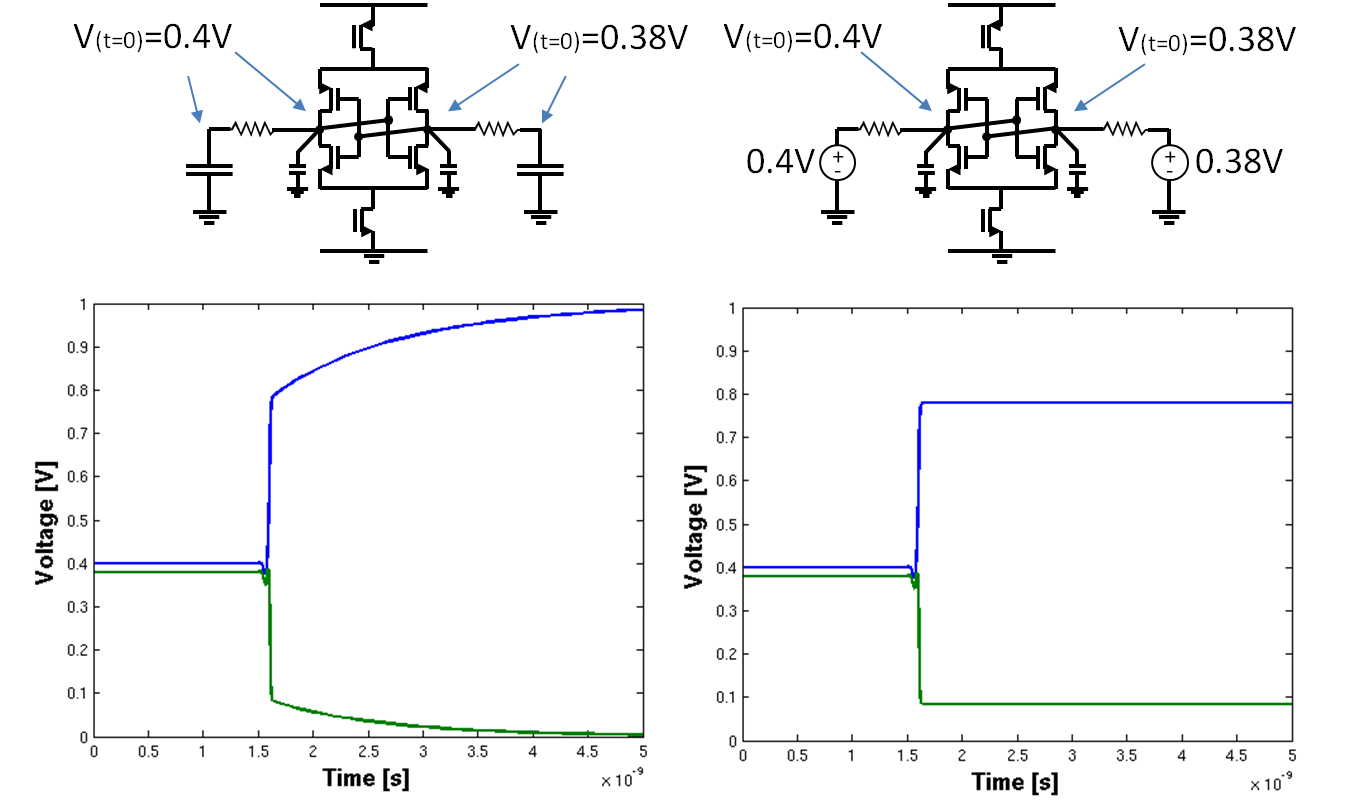
\includegraphics[width=\textwidth]{../fig/hfdstk-sensamp-RC-latch-explain.png}
  \caption{Vergelijking situatie met voorgeladen (eindige) capaciteit en situatie met spanningsbron (oneindige capaciteit)}
  \label{fig:RC-latch-explain}
\end{figure}
Gevolgen van wanneer dit effect optreedt is dus dat het nuttige signaal zich snel - alsof er helemaal geen last aanhangt - en lineair opbouwt en dat er geen AC-signaal is over de condensator. Een analyse van de respons van een RC-circuit op een lineair stijgende spanningsbron geeft meer duidelijkheid voor de voorwaarden waarop het RC-latch-effect optreedt (zie figuur \ref{fig:RC-latch-maplecircuit}). De respons van de spanning over de capaciteit is $Vcap(t) =  at - aRC(1-e^{-{\frac {t}{CR}}})$. Uit deze uitdrukking blijkt dat het RC-latch-effect optreedt wanneer de latch zonder latch snel is (a<<1) en/of wanneer het RC-product hoog is (RC>>1).
Wanneer het effect zich voordoet zijn latching en RC-respons onafhankelijke processen. Wanneer de voorwaarden niet meer zo uitgesproken zijn, gaan deze processen met elkaar interfereren en is het moeilijk dit gecombineerde proces wiskundig te beschrijven.
\begin{figure}
  \centering
  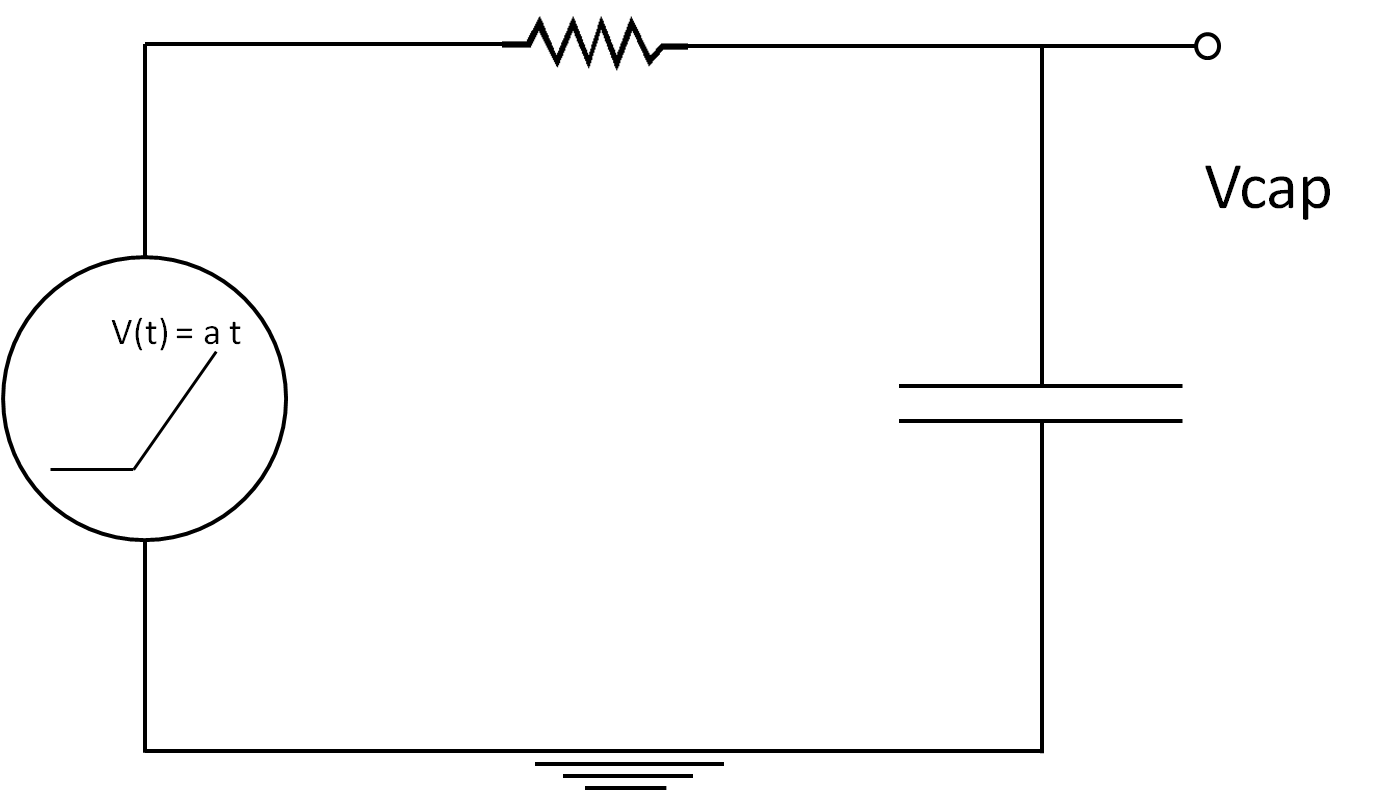
\includegraphics[scale=0.4]{../fig/hfdstk-sensamp-RC-latch-maplecircuit.png}
  \caption{Circuit voor analyse voorwaarden RC-latch-effect}
  \label{fig:RC-latch-maplecircuit}
\end{figure}

Conclusie van het RC-latch effect is dat de timing helemaal niet zo kritisch is: in theorie hoeft de overlap slechts even lang te duren als de delay van de SA wanneer er geen last op is aangesloten, maar het is niet erg als de overlap wat langer duurt.
De pass-gates mogen ook minimaal zijn, om hun aanweerstand te vergroten zodat het effect kan optreden.
In geval verder zou gewerkt worden met een SA zonder overlap met pass-gate-enable en SA-enable, zouden de pass-gates moeten geschaald worden om de mismatch te minimaliseren. Dit zou wel betekenen dat er per schakeling


\subsection{Sensitiviteitsanalyse voor minimale SA - vervolg}

In tabel \ref{tab:min-sensanalysis-overlap} worden de resultaten van een nieuwe sensitiveitsanalyse getoond voor een minimale SA, ditmaal waarbij er dus overlap is tussen pass-gate-enable en SA-enable. In deze situatie dragen de pass-gates amper bij tot de offsetspanning. 
Vooral de transistors van de differentiele paren zullen opgeschaald moeten worden om de offsetspanning in te perken, de andere transistoren schalen zal invloed hebben op snelheid en energie.

\subsection{Sensitiviteitsanalyse voor gebruikte SA}

In tabel \ref{tab:ourSA-sensanalysis-overlap} worden de resultaten van een sensitiviteitsanalyse getoond voor de SA die gebruikt wordt in het finale geheugenontwerp. Deze is gekozen aan de hand van de resultaten van de paretosimulatie in de volgende sectie.


\section{Paretosimulatie}
In het beginstadium van het ontwerp is nog niet duidelijk wat de impedantie aan de BL wordt. Het is deze impedantie die bepaalt wat het spanningsverschil is tussen het datasignaal en het referentiesignaal aan de sense amplifier. Bovendien kan het zijn dat er midden in het ontwerp besloten wordt om een andere impedantie te kiezen om alsnog te optimaliseren naar een andere variabele.
Natuurlijk is het mogelijk om één SA te gebruiken die voor elke impedantie een correcte en snelle werking zou garanderen. Dit zou echter een verspilling zijn van energie. In deze sectie wordt een pareto-oppervlak opgesteld waarbij er voor elk spanningsverschil de snelste en energiezuinigste SA-ontwerpen worden gekozen.

\subsection{Opstelling}
Uit een verzameling van allerhande SA [dit zijn sense amplifiers waarvan de transistoren verschillend geschaald zijn - differentiele paren hebben zelfde afmetingen] worden enkel de pareto-optimale SA uitgekozen. De pareto-criteria zijn $\Delta V$, snelheid en dynamische energie. 

Voor deze opstelling worden de pass-gates weggelaten van de SA [dit is geoorloofd zoals bleek uit de sensitiviteitsanalyse], de last aan de ingangs-uitgangsknopen is een simpele CMOS inverter. De knopen zijn voorgeladen op 2 spanningen: 0,4V en 0,4V - $\Delta V$. Na 0,5ns wordt de SA aangezet en wordt de tijd gemeten tot wanneer de ingangs-uitgangsknopen geladen of ontladen zijn tot 99,9\% van hun finale waarde (VDD of VSS). Dit is wellicht een te strenge methode om de snelheid van de SA te bepalen aangezien de inverters al eerder zullen schakelen. Indien de snelheid van de 2 knopen verschilt, zal de traagste tijd genomen worden. De dynamische energie wordt opgemeten van het moment dat de SA wordt aangeschakeld tot dit tijdstip. Ook het statisch vermogen van de SA wordt opgemeten wanneer de ingangs-uitgangsknopen VDD en VSS bereikten. Uiteraard wordt ook geverifieerd ofdat de SA wel correct heeft gelatcht.

Per sense amplifier worden er 250 Monte Carlo simulaties gedaan met deze opstelling. Indien de SA niet elke keer correct functioneerde, wordt de SA verworpen. Latchte de SA wel elke keer correct, wordt het gemiddelde van de delay, dynamische energie  en statisch vermogen opgeslagen. 

\subsection{Resultaten}
Op figuur \ref{fig:pareto} zijn de pareto-optimale resultaten getoond van de groep sense amplifiers. Het doel van deze simulatie is veeleer om de transistorafmetingen te situeren in functie van deze optimalizatievariabelen. Voor deze simulatieopstelling kan men enkel zeggen dat de kans dat de offsetspanning lager is dan $\Delta V$ minstens $1 -\frac{1}{250}$ is. Dit is een veel te kleine garantie voor een sense amplifier die misschien wel miljoenen keren zal gefabriceerd worden. Voor meer informatie over de verdeling van de offsetspanning te krijgen moet de standaardafwijking berekend worden met de sensitiviteitsanalyse.

\begin{figure}
  \centering
  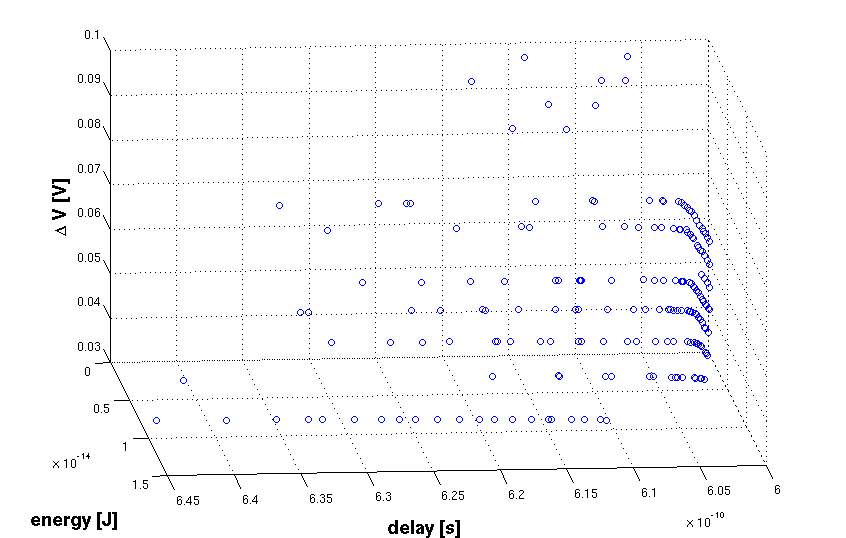
\includegraphics[scale=0.4]{../fig/hfdstk-sensamp-pareto.png}
  \caption{De pareto-optimale sense amplifiers}
  \label{fig:pareto}
\end{figure}

\section{Besluit}
In dit hoofdstuk werd dieper ingegaan op de sense amplifiers, die het kleine spanningsverschil tussen datasignaal en referentiesignaal correct moet versterken tot VDD en VSS. De belangrijkste eigenschap van de SA is de offsetspanning door transistorvariaties. Deze kan voldoende klein gemaakt worden door de transistoren voldoende op te schalen. De offsetspanning kan statistisch beschreven worden met behulp van een sensitiviteitsanalyse. Tenslotte worden er ook uit een grote groep SA de pareto-optimale gekozen. De resultaten geven een idee van de grootteordes van transistorafmetingen voor een bepaalde offetspanning, snelheid en dynamische energie.

\chapter{Omringende logica}
\label{periphery}

Het geheugensysteem maakt gebruik van bouwblokken zoals decoders, buffers en passgates.
In dit hoofdstuk worden deze componenten van naderbij onderzocht.

\section{Decoders}
Een decoder is een logsiche schakeling: op basis van een geëncodeerde bus van ingangen brengt de decoder één uitgang actief hoog; uit een combinatie van N ingangen, gaat er steeds één van $2^N$ uitgangen actief hoog worden\footnote{Er is nog een enable-controlesignaal, wanneer dit actief laag is, worden alle uitgangen laag.}. Om alle mogelijke geheugenconfiguraties (aantal WLs en BLs) te kunnen exploreren in sectie \ref{optimization}, werd er een gamma aan decoders ontworpen gaande van een 2-naar-4 decoder tot en met een 9-naar-512 decoder. Grotere decoders worden opgebouwd uit kleinere decoders. Dit kan gedaan worden op 2 manieren; volgens een boompatroon (\ref{fig:decoder1}) of volgens een gridpatroon (\ref{fig:decoder2}). In de volgende secties wordt het ontwerp van beide manieren toegelicht en vergeleken.

\begin{figure}[!ht]
\centering
\subfloat[Tree decoder]{ 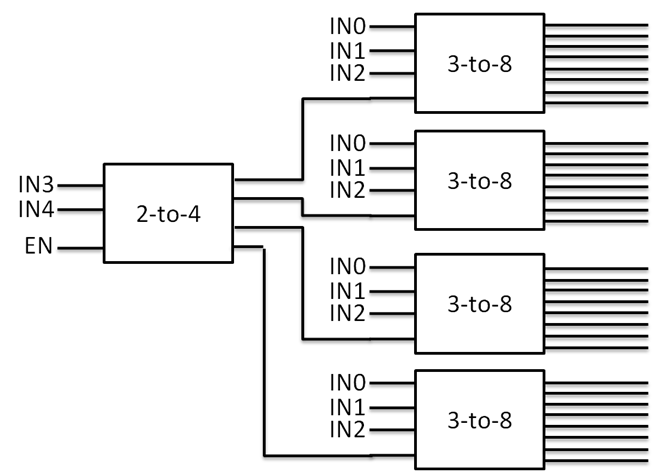
\includegraphics[width=0.45\textwidth] {../fig/hfdst-decoders-type1.png} \label{fig:decoder1}}
\subfloat[Grid decoder]{ 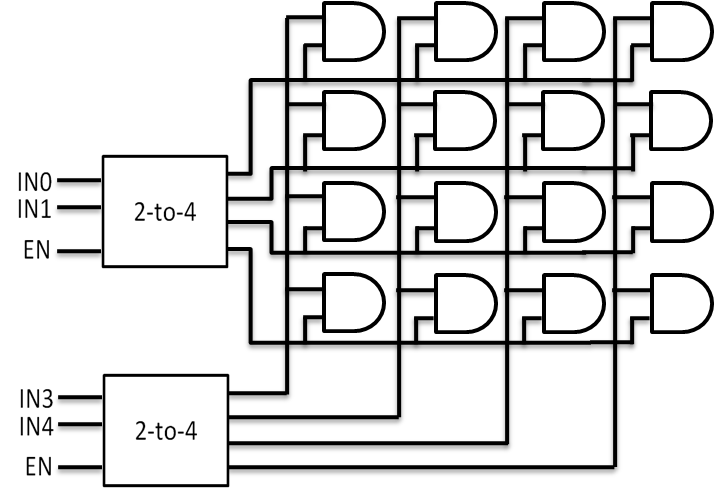
\includegraphics[width=0.45\textwidth] {../fig/hfdst-decoders-type2.png} \label{fig:decoder2}}
\caption[Types decoders]{Opbouw voor grotere decoders}\label{fig:basisdecoders}
\end{figure}

\subsection{De tree decoder}
De tree decoder is een decoder met een meerlaagse structuur die zich uitwaaiert naar de uitgangen. De basisblokken van deze decoder zijn een 2-naar-4 decoder (figuur \ref{fig:decoder2to4}) en een 3-naar-8 decoder (figuur \ref{fig:decoder3to8}). Het principe van de tree decoder is als volgt: met x-naar-$2^x$ en y-naar-$2^y$ decoders kan men een $x+y$-naar-$2^{x+y}$ realiseren door ze te cascaderen. De MSBs worden aangesloten aan de eerste laag. Dit wordt geïllustreerd in de vorm van een 5-naar-32 decoder in figuur \ref{fig:decoder1}. 
\begin{figure}[!ht]
\centering
\subfloat[2-naar-4 decoder]{ 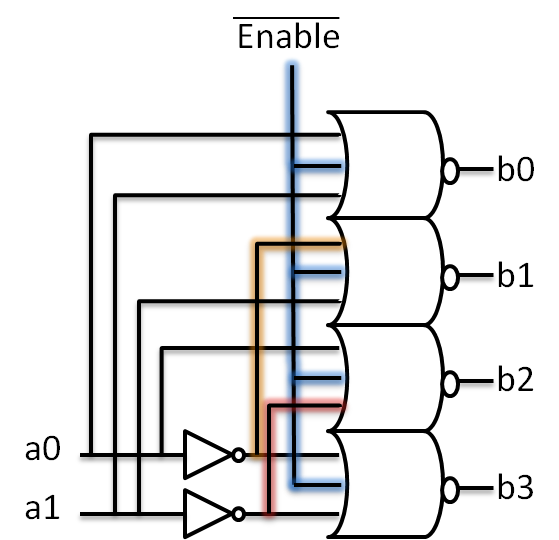
\includegraphics[width=0.5\textwidth] {../fig/hfdst-decoders-2to4.png} \label{fig:decoder2to4}}
\subfloat[3-naar-8 decoder]{ 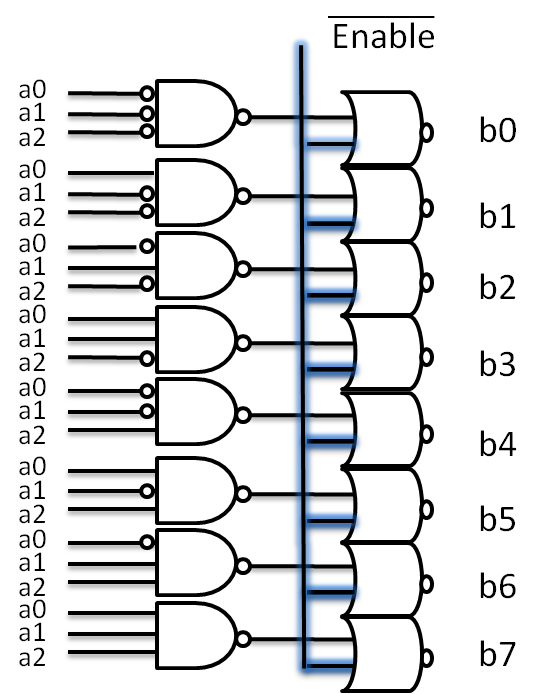
\includegraphics[width=0.5\textwidth] {../fig/hfdst-decoders-3to8.png} \label{fig:decoder3to8}}
\caption[Basis decoders]{Basis decoders}
\end{figure}

\subsection{De grid decoder}
De grid decoder heeft een tweelaagse structuur. De eerste laag bestaat uit een aantal 2-naar-4 en/of 3-naar-8 decoders die in parallel staan. De verschillende uitgangen van deze eerste laag worden dan met AND-gates samen gevoegd in een tweede laag. Om glitches te voorkomen is het belangrijk dat al de signalen gelijktijdig binnen komen in de AND-gates, daarom werd de topologie van de 2-naar-4 decoder van figuur \ref{fig:decoder2to4} veranderd tot een NAND-NOR topologie zoals die van de 3-naar-8 decoder in figuur \ref{fig:decoder3to8}. Bij grotere decoders worden de uitgangen van de eerste laag aangesloten aan een groot aantal AND-gates. Omwille van deze grote fan-out moeten de uitgangen van de eerste laag gebufferd worden met overeenkomstig geschaalde inverters. Omdat er dus toch al minstens 2 inverters voor de AND-gates worden geplaatst, worden deze geïmplementeerd als NOT-gate + NOR-poort i.p.v. NAND-poort + NOT-poort. Op deze manier wordt er één inverter uitgespaard. Tabel \ref{tab:griddecoder} geeft de hoeveelheid basisdecoders weer in de eerste laag van de grid decoder en het aantal AND-gates de tweede laag, in functie van het aantal inputs.

\begin{table}
\begin{center}
\begin{tabular}{llll}
\hline
\# inputs decoder & \# 2-naar-4 decoders & \# 3-naar-8 decoders & \# AND-gates\\
\hline
4 & 2 & 0 & 16\\
5 & 1 & 1 & 32\\
6 & 0 & 2 & 64\\
7 & 2 & 1 & 128\\
8 & 1 & 2 & 256\\
9 & 0 & 3 & 512\\
\hline
\end{tabular}
\end{center}
\caption[Aantal gates in de grid decoder]{Aantal gates in de grid decoder}
\label{tab:griddecoder}
\end{table}

\subsection{Vergelijkende studie}
Eens ontworpen, kunnen de tree en grid decoders met elkaar vergeleken worden. Naast oppervlakte, energie en delay worden ook glitches, mismatch en delay tussen verschillende addressen onderzocht. \\
Zoals in figuur \ref{fig:decoder_a} gezien kan worden, schaalt de oppervlakte van de grid decoder veel minder dan die van de tree decoder bij een groot aantal ingangen. De plotse stijging in de oppervlakte van de tree decoder met 8 ingangen kan verklaard worden door het gebruik van een extra laag in de boomstructuur. \\
Het energieverbruik wordt vergeleken in figuur \ref{fig:decoder_e}. De grid decoder verbruikt minder energie in functie van het aantal ingangen. Sommige signalen in de tree decoder zullen diep doorrimpelen, waardoor er meer gates zullen schakelen dan in de grid decoder.  Het overbodig schakelgedrag van de tree decoder zou tot op zekere hoogte ingeperkt kunnen worden door de topologie van de basisdecoders (figuur \ref{fig:basisdecoders}) te wijzigen zodat de enable vooraan komt te staan.\\
De delay van de decoders kan afgelezen worden in figuur \ref{fig:decoder_d}. Beide types decoders hebben ongeveer dezelfde delay. Bij grotere grid decoders kan de extra delay verklaard worden door de extra latency van de buffers.\\
Verder werden glitches onderzocht. In beide types decoders kunnen er glitches opduiken. De oorsprong van dit probleem ligt bij het gebuik van de NOR-gates. Wanneer de twee ingangs-signalen van de NOR-gate niet gelijktijdig toekomen (zie figuur \ref{fig:decoder_glitch}), kan de uitgang van de gate tijdelijk actief hoog getrokken worden, om vervolgens weer laag getrokken te worden. Bij de tree decoder is het nagenoeg onmogelijk om deze ongelijktijdigheid te voorkomen: sommige signalen moeten immers meer lagen doorlopen dan andere vooraleer de NOR-ingang bereikt wordt. Bij de grid decoder kan een glitch opduiken als de buffers die de tweede laag aansturen een asymmetische delay hebben. Dit kan bijvoorbeeld voorkomen bij een 5-naar-32 decoder. De uitgangen van de 2-naar-4 decoder en de 3-naar 8-decoder in deze decoder hebben een andere last. Sommige buffers kunnen echter suboptimaal ontworpen worden zodat de NOR-ingangssignalen alsnog ongeveer gelijktijdig toekomen.\\
Na een snelle mismatch-analyse blijkt dat de grid decoder minder variatie toont in dynamisch energieverbruik en delay dan de tree decoder. Tenslotte heeft de tree decoder een grotere spreiding wat delay betreft, afhankelijk van het vorige en huidige addres: wanneer er slechts één adresbit schakelt, kan het voorkomen dat dit signaal slechts kort moet doorrimpelen tot de uitgang. Dit ziet men minder in de grid decoder. \\
Na het vergelijken van beide decoders wat oppervlakte, energie, delay, glitches, mismatch en delay betreft, komt de grid decoder er als beste uit en zal deze dan ook gebruikt worden in het finale ontwerp.


\begin{figure}[!ht]
\centering
\subfloat[Oppervlakte]{ 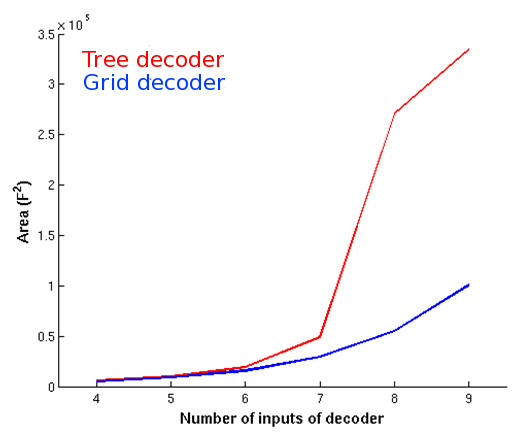
\includegraphics[width=0.5\textwidth] {../fig/hfdst-decoders-a.png} \label{fig:decoder_a}}
\subfloat[Energie]{ 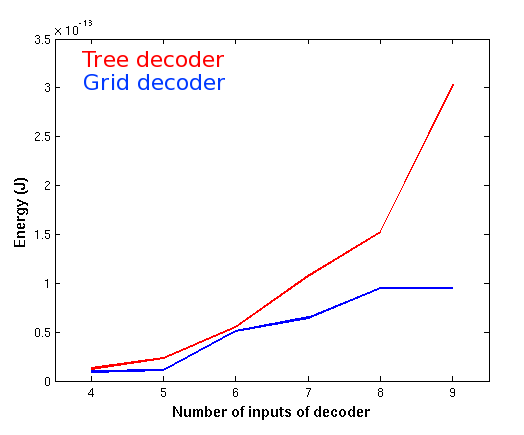
\includegraphics[width=0.5\textwidth] {../fig/hfdst-decoders-e.png} \label{fig:decoder_e}}\\
\subfloat[Delay]{ 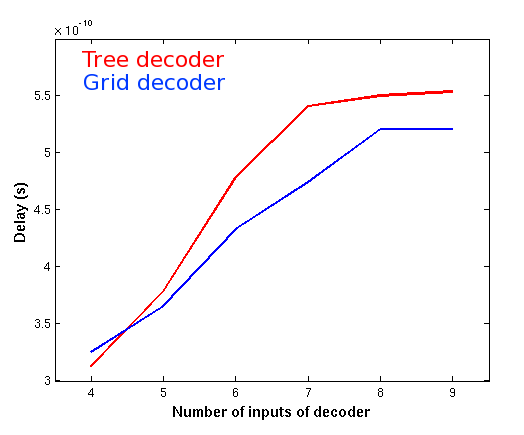
\includegraphics[width=0.5\textwidth] {../fig/hfdst-decoders-d.png} \label{fig:decoder_d}}
\caption[Vergelijking van decoder types]{Vergelijking van decoder types}
\end{figure}


%\begin{figure}[!ht]
%  \centering
%  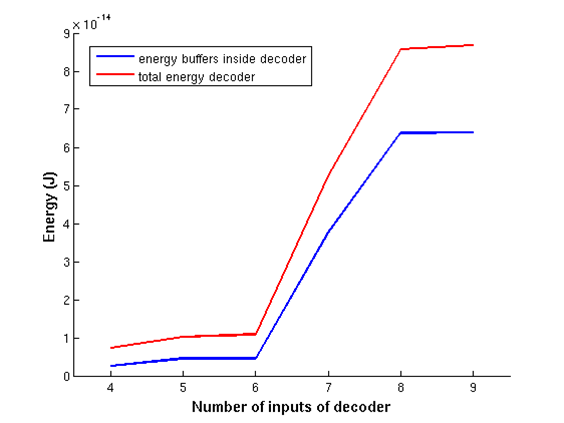
\includegraphics[width=0.8\textwidth]{../fig/hfdst-decoders-egrid.png}
%  \caption{Energie verbruik in griddecoder}
%  \label{fig:decoder_egrid}
%\end{figure}

\begin{figure}[!ht]
  \centering
  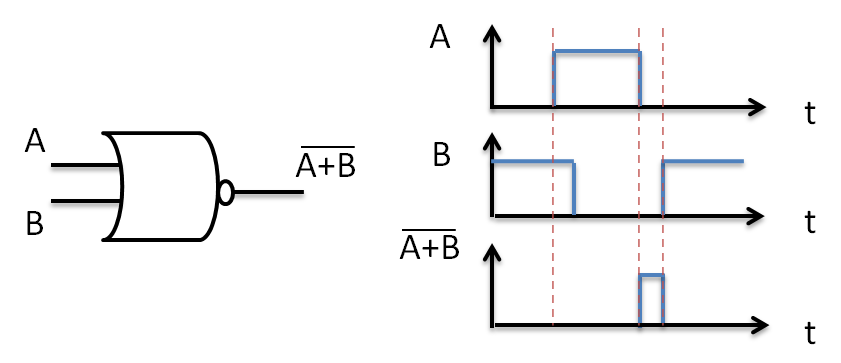
\includegraphics[width=0.8\textwidth]{../fig/hfdst-decoders-glitch.png}
  \caption[Glitch in NOR-gate]{Glitch in NOR-gate}
  \label{fig:decoder_glitch}
\end{figure}


\section{Buffers}
Kleine CMOS gates kunnen slechts een beperkte hoeveelheid stroom leveren. Wanneer de uitgang van deze gates aangesloten wordt op een grote capacitieve last, duurt het lang voordat deze last op- of ontladen is. Soms is het niet aangewezen om deze gate zelf te vergroten, hierdoor neemt de intrinsieke last immers toe en gaan de gates van de vorige trap mogelijk niet meer genoeg stroom kunnen leveren om de ingang van de gate snel te sturen. In dit geval is het aangewezen om de uitgang van de gate te bufferen. Een ideale buffer heeft geen ingangscapaciteit en kan oneindig veel stroom leveren om eender welke last onmiddelijk te sturen. In de praktijk worden buffers geïmplementeerd door een even aantal invertoren te cascaderen. De eerste inverter in de ketting is klein genoeg zodat de gebufferde gate hier geen last van ondervindt, de volgende inverters in de ketting worden systematisch opgeschaald zodat de laatste inverter in de ketting voldoende stroom kan leveren om de last te sturen. 
Buffers worden op drie plaatsen in de geheugen architectuur gebruikt. Ten eerste om de woordlijnen aan te sturen. Ten tweede om de referentielogica aan te sturen en tenslotte  tussen de eerste en tweede laag in de grid decoders. Tabel \ref{tab:buffer} geeft een overzicht van de oorsprong van de last en de waarde van de last die de verschillende buffers moeten aansturen.\\
De buffers werden ontworpen met de methode van logical effort\cite{Sutherland:1999:LED:298513} waarbij het aantal stages en de sizing van elke stage werd bepaald volgens het volgende stappenplan:
\begin{enumerate}
\item Bepaal de path effort $F = GH$ waarbij $G = 1$ aangezien we enkel met inverters werken en $H = \frac{C_{out}}{C_{in}}$
\item Het aantal stages wordt bepaald door $\hat{N} = log_{4}F$. Hierbij werd er voor een stage effort van 4 gekozen voor een optimale delay. \^{N} wordt dan afgerond tot een even getal N voor de woordlijn- en referentiebuffers en tot een oneven getal voor de decoderbuffers.
\item N wordt dan gebruikt om een nieuwe stage effort \^{f} te berekenen met de formule $\hat{f} = F^{1/N}$.
\item Tenslotte kunnen de groottes van de verschillende invertoren in de chain berekend worden met de nieuwe stage effort $\hat{f} = gh$.
\end{enumerate}
Figuur \ref{fig:refbuffer} illusteert de ongebufferde en gebufferde signalen die naar de referentielogica gaan, voor verschillende veelvouden van elementaire last (een NOR-gate en een NOT-gate).

\begin{table}
\begin{center}
\begin{tabular}{ccc}
\hline
 &  Last & \ Capaciteit\\
\hline
Woordlijnbuffer & 1 Transistorgate &  $\#BL*0,18fF$\\
Referentiebuffer & 1 Nor + 1 Inv &  $\#BL*0,93fF$\\
Decoderbuffer & 1 Nor & (4-64)\footnote{varieert met machten van 2, hangt af van hoeveel uitgangen de decoder bevat}$*0.58fF$\\
\hline
\end{tabular}
\end{center}
\caption[Lasten aangedreven door de verschillende buffers]{Lasten aangedreven door de verschillende buffers}
\label{tab:buffer}
\end{table}

\begin{figure}[!ht]
  \centering
  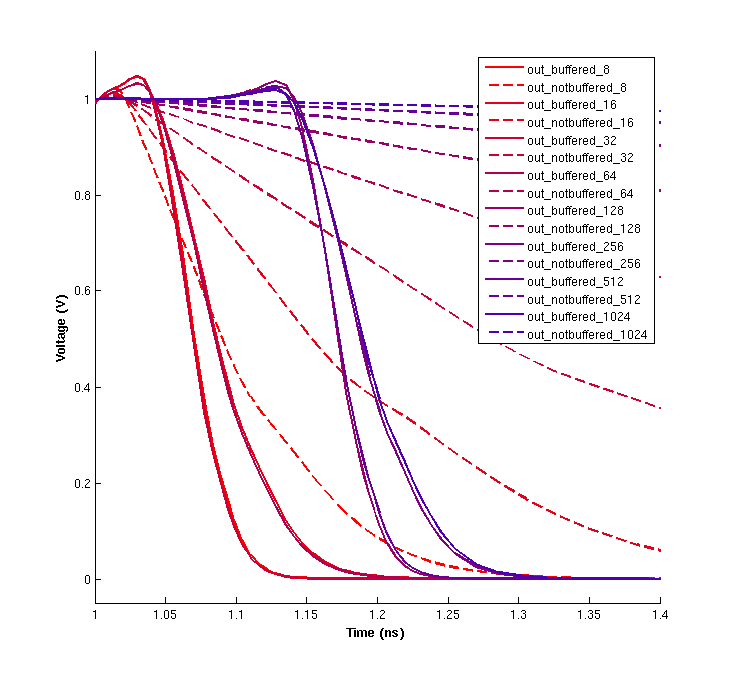
\includegraphics[width=0.8\textwidth]{../fig/hfdst-buffers-refbuffer.png}
  \caption[Gebufferde en ongebufferde signalen naar de referentie logica]{Gebufferde en ongebufferde signalen naar de referentie logica - ongebufferde signalen ontladen traag door de zware last, buffers kunnen snel deze last ontladen/opladen. Er zit vertaging op het signaal op heel zware lasten omdat de buffer bestaat uit een groot aantal inverters}
  \label{fig:refbuffer}
\end{figure}

\section{BL en WL drivers}
Elk global block (GB) heeft ingangslijnen voor geëncodeerde BL- en WL-signalen. Het zou energieverspilling zijn om deze signalen naar alle GB te laten propageren, terwijl er slechts 1 GB in werking zal treden omdat het bijhorende $GB\_{Enable}$-controlesignaal actief hoog is. Deze vertakte lijnen, die over heel de chip lopen zouden immers onnodig een aanzienlijke capaciteit opladen (zie figuur \ref{fig:nodrivers}). Het is beter om deze BL- en WL-signalen tussenin nog te laten bufferen zoals op figuur \ref{fig:drivers}. Deze drivers kunnen eenvoudig gerealiseerd worden met AND-gates in een NAND-gate + NOT-gate implementatie.
De energiewinst hangt natuurlijk samen met de onwerpparameters NoGB, NoBLpLB en NoWLpB: er zijn NoGB $GB\_{Enable}$ signalen, die elk $\log_2 NoBLpLB +\log_2 NoWLpB$ drivers moeten aansturen. Deze extra benodigde energie moet kleiner zijn dan de energie die wordt gewonnen door een groot deel capaciteit van de lijnen te vermijden. Exacte waardes voor deze capaciteiten kunnen maar worden bepaald door parasitaire layout extraction, wat in dit werk niet is uitgevoerd.

\begin{figure}[h!]
  \centering
  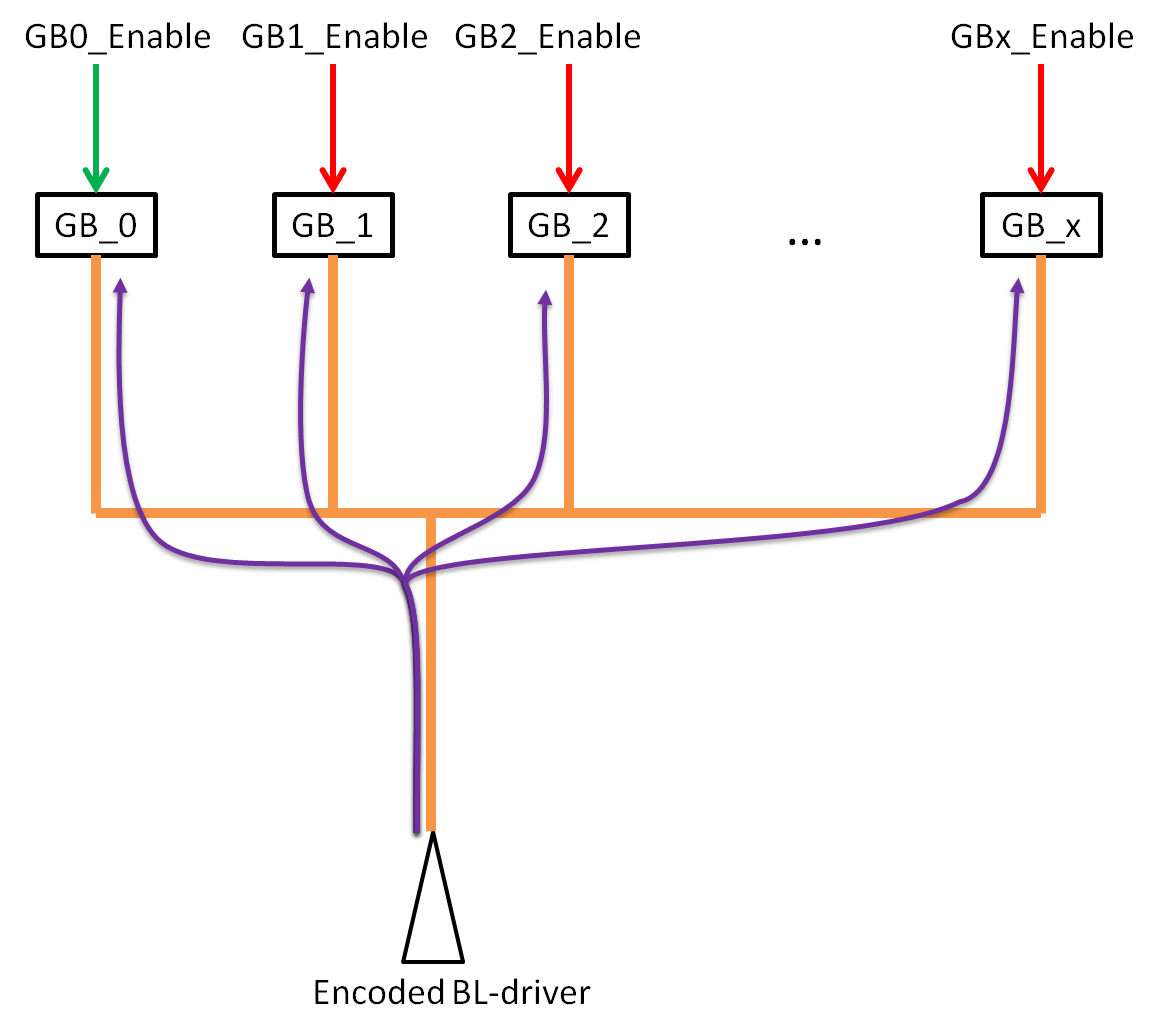
\includegraphics[width=0.5\textwidth]{../fig/hfdstk-periphery-nodrivers.png}
  \caption[BL- en WL-drivers]{Off-chip driver moet onnodig veel last opladen}
  \label{fig:nodrivers}
\end{figure}
\begin{figure}[h!]
  \centering
  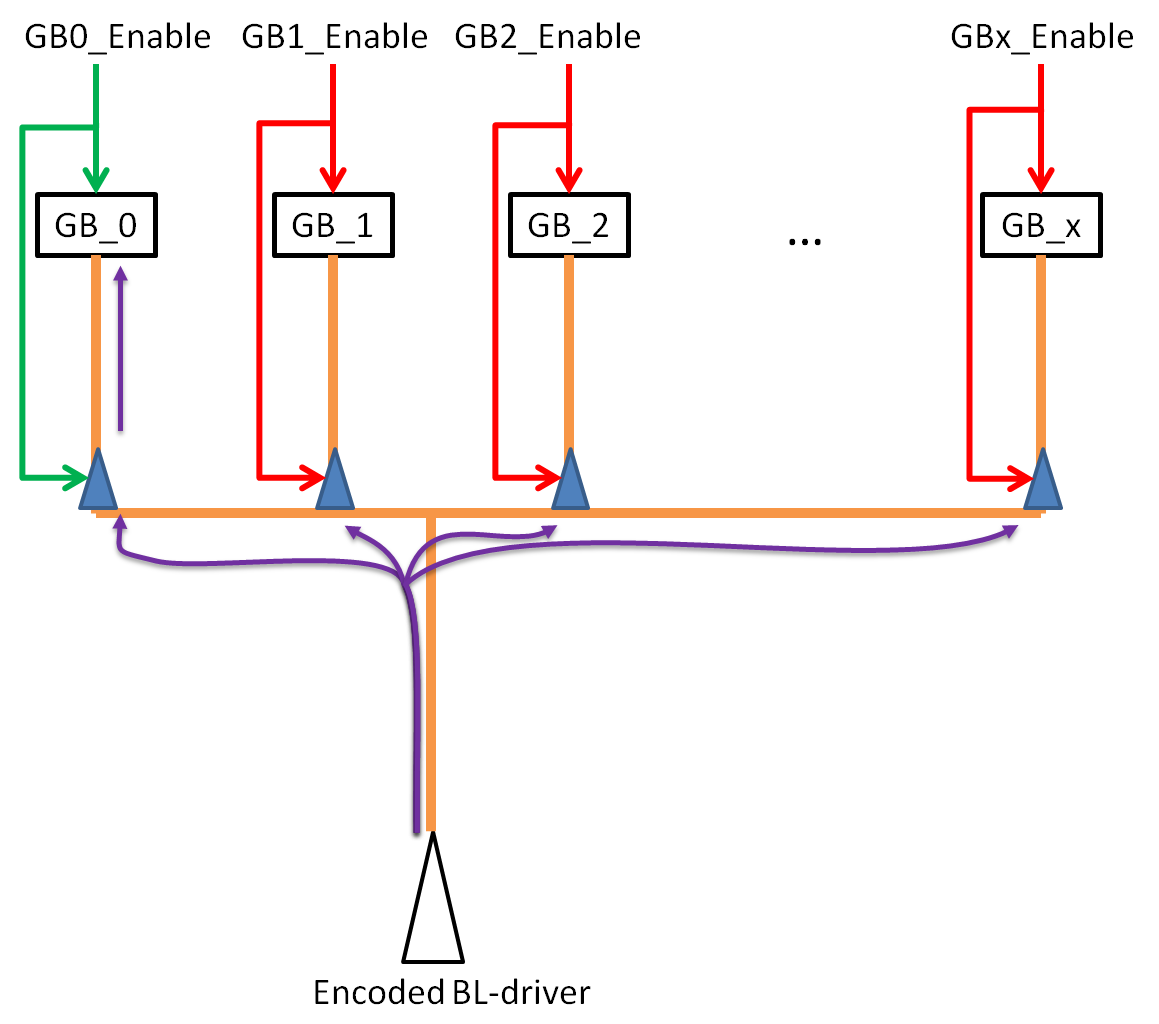
\includegraphics[width=0.5\textwidth]{../fig/hfdstk-periphery-drivers.png}
  \caption[BL- en WL-drivers]{Tussenin wordt gebufferd, zodat niet hele lijnen moeten worden opgeladen}
  \label{fig:drivers}
\end{figure}

\section{Passgates}
Passgates zijn schakelaars die de spanning van een laagimpedant knooppunt doorlaten naar een hoogimpedant knooppunt. Idealiter heeft de passgate geen weerstand wanneer hij aanstaat. In de praktijk zal er altijd een beetje weerstand zijn, dit heeft als gevolg dat er een kleine RC-delay vooraleer het hoogimpedante punt is geladen/ontladen tot de waarde van het laagimpedante punt.
Een passgate kan gerealiseerd worden met een nMOS transistor, een pMOS of een combinatie van beiden.
In wat volgt worden de verschillende scenario's besproken die kunnen optreden wanneer de schakelaar aangezet wordt, de passgate zal immers niet altijd stroom kunnen leveren om het hoogimpedante knooppunt te (ont)laden.

\subsection{nMOS passgate}
De opstelling is het circuit van figuur \ref{fig:passgate1}. Afhankelijk van de (initiële) waardes van Vx en Vs, kunnen volgende situaties optreden.

\begin{figure}[h!]
  \centering
  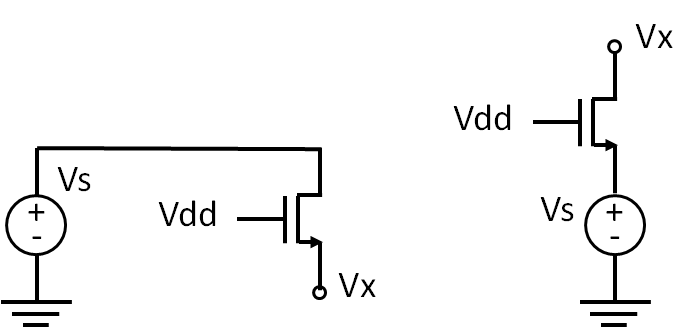
\includegraphics[width=0.5\textwidth]{../fig/hfdst-periphery-passgate1.png}
  \caption[nMOS passgate]{nMOS passgate opstelling. a: Vs > Vx, b: Vs < Vx}
  \label{fig:passgate1}
\end{figure}

\begin{itemize}
\item Vx > Vs en Vdd - Vs > Vtn: de transistor ontlaadt Vx tot Vs.
\item Vx > Vs en Vdd - Vs < Vtn: de transistor staat af, er gebeurt niets.
\item Vx < Vs en Vs < Vdd - Vtn: de transistor levert stroom tot Vx is opgeladen tot Vs.
\item Vx < Vs, Vs > Vdd - Vtn en Vx < Vdd - Vtn: de transistor gaat Vx opladen tot Vdd - Vtn.
\item Vx < Vs, Vs > Vdd - Vtn en Vx > Vdd - Vtn: de transistor staat af, er gebeurt niets.
\end{itemize}

\subsection{pMOS passgate}
De opstelling is het circuit van figuur \ref{fig:passgate2}. Er kunnen wederom verschillende situaties optreden.

\begin{figure}[h!]
  \centering
  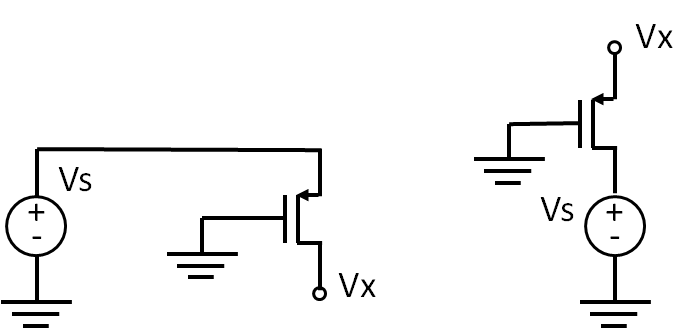
\includegraphics[width=0.5\textwidth]{../fig/hfdst-periphery-passgate2.png}
  \caption[pMOS passgate]{pMOS passgate opstelling. a: Vs > Vx, b: Vs < Vx}
  \label{fig:passgate2}
\end{figure}

\begin{itemize}
\item Vs > Vx en Vs > |Vtp|: de transistor laadt Vx op tot Vs.
\item Vs > Vx en Vs < |Vtp|: de transistor staat af, er gebeurt niets.
\item Vs < Vx en Vs > |Vtp|: de transistor levert stroom tot Vx is ontladen tot Vs.
\item Vs < Vx, Vs < |Vtn| en Vx > |Vtp|: de transistor gaat Vx ontladen tot |Vtp|.
\item Vs < Vx, Vs < |Vtn| en Vx < |Vtn|: de transistor staat af, er gebeurt niets.
\end{itemize}

Er zijn dus spanningszones waarvoor de passgate niet functioneert. Het is belangrijk te weten wat deze zones zijn, zodat het circuit ontworpen wordt om deze zones te vermijden. 
Op figuur \ref{fig:passgate3} worden deze zones in kaart gebracht voor een nMOS, een pMOS en een complementaire passgate, zowel voor LVT als HVT transistoren. De resultaten komen voort uit een transiënte simulatie van 1 ns, de bijdrage van lekstromen is op deze korte tijd verwaarloosbaar. Er dient opgemerkt te worden dat de passgates niet (of slechts even) aanstaan voor sommige zones, maar dat de uiteindelijke fout nog meevalt.
Als Vs bijvoorbeeld 0,9V bedraagt voor een nMOS passgate en Vx initieel 0,85V (met Vdd 1V), levert de transistor geen stroom, maar bedraagt de uiteindelijke fout 'slechts' 50mV.
In deze fout zit nog geen ladingsinjectie inbegrepen, eenmaal de passgate afschakelt is de injectie onvermijdelijk.
Zowel de LVT als de HVT complementaire passgates vertonen geen dode zones. Voor performantieredenen is geopteerd voor de LVT transistoren in het geheugenontwerp.

\begin{figure}[!ht]
\centering
\subfloat[CLVT]{ 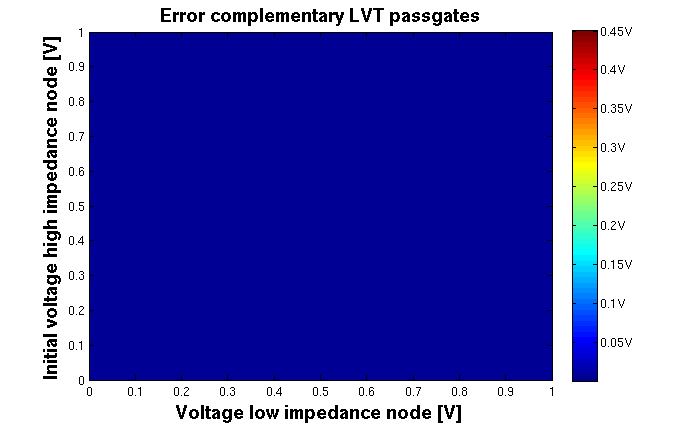
\includegraphics[width=0.5\textwidth] {../fig/hfdstk-periphery-CLVT.png}}
\subfloat[CHVT]{ 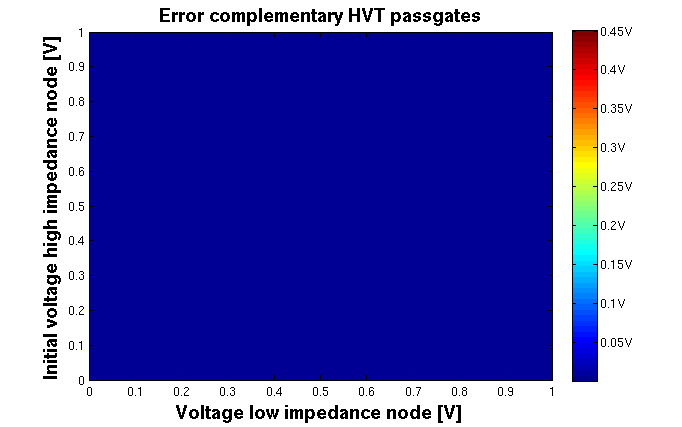
\includegraphics[width=0.5\textwidth] {../fig/hfdstk-periphery-CHVT.png}}\\
\subfloat[NLVT]{ 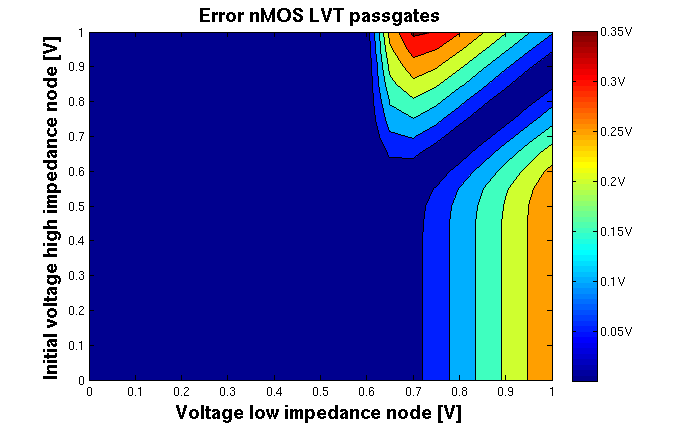
\includegraphics[width=0.5\textwidth] {../fig/hfdstk-periphery-NLVT.png}}
\subfloat[NHVT]{ 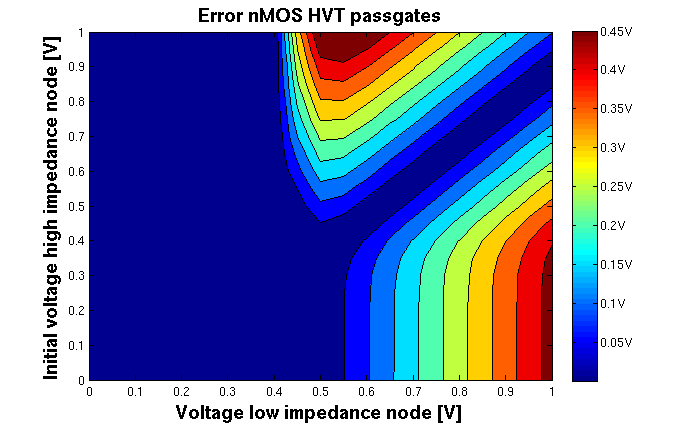
\includegraphics[width=0.5\textwidth] {../fig/hfdstk-periphery-NHVT.png}}\\
\subfloat[PLVT]{ \includegraphics[width=0.5\textwidth] {../fig/hfdstk-periphery-PLVT.png}}
\subfloat[PHVT]{ \includegraphics[width=0.5\textwidth] {../fig/hfdstk-periphery-PHVT.png}}
\caption[Dode zones voor verschillende types passgates]{Dode zones voor verschillende types passgates - de contouren stellen het verschil voor tussen Vs en Vx na 1 ns}
\label{fig:passgate3}
\end{figure}



\section{Besluit}
Bij het ontwerpen van een geheugen is er nood aan een aantal logische bouwblokken: decoder, buffers, passgates. Ontwerpproblemen en -keuzes werden geanalyseerd en toegelicht. Bij de decoders werd er gekozen voor een grid architectuur om glitches te vermijden. Buffers werden ontworpen op basis van logical effort, waarbij het aantal trappen werd bepaald in functie van de last. En tenslotte bleek uit de analyse van de passgates dat er nood was aan complementaire pass-gates met lage Vt.

\chapter{Timing en optimalizatie}
\label{timing-optimization}
Voor een correcte werking van het geheugen, is het van belang dat de verschillende controlesignalen in een bepaalde volgorde verwerkt en doorgegeven worden.
In dit hoofdstuk zal toegelicht worden welke deze timingvoorwaarden zijn en met welke technieken deze voorwaarden gerealiseerd kunnen worden.
Ook wordt er besproken welke invloed de vrijheidsgraden van hoofdstuk \ref{architecture} hebben op de resulterende totale snelheid, energie en oppervlakte van het totale systeem. 

\section{Timing in het Local Block}

\section{Analyse verschillende geheugenconfiguraties}


\section{Besluit}

\chapter{Volledige ontwerp}
\label{final}
\section{Het finaal ontwerp}
Het finale ontwerp is een geheugen dat uit 32BL, 32WL en 512GB bestaat. Van de 32 BL worden er 16 gebruikt voor het genereren van het referentiespanning. En van de 16 gebruikte cellen zijn er 6 in HRS en 10 en LRS. Dit om de referentiespanningsverdeling beter te centreren tussen de BL-spanningen voor cellen in RHS en LRS. De afmetingen van alle transistoren staan in tabel \ref{tab:transsize}. \\
Op dit geheugen wordt een speed-vdd-test uitgevoerd. Dit is een test waarbij de voedingspanning wordt verlaagd en er vervolgens geverifieerd wordt aan welke snelheid de leescyclus nog kan uitgevoerd worden. Hierbij wordt de dutycycle spanningsdeling-latching manueel gekozen op basis van het circuitgedrag op de voedingspanning. Dit geeft natuurlijk een meer optimistisch beeld dan dat er een kloksignaal met een bepaalde frequentie zou verwerkt worden door digitale logica om deze dutycycle te bekomen. De delay van de logica zou overigens niet lineair schalen met de voedingspanning, waardoor de dutycycle sowieso niet constant blijft. Figuur \ref{fig:speedvdd} toont de resultaten van deze test. Voor elk vakje in de shmoo plot werden 100 Monte Carlo simulaties uitgevoerd, een groen vakje stelt 100 geslaagde leesoperaties voor, bij een rood vakje is er minstens 1 leescyclus foutief verlopen. Zoals men duidelijk kan zien  daalt de leessnelheid bij het verlagen van de voedingspanning. Dit komt door een combinatie van 2 factoren. Ten eerste gaat de logica trager worden, dit heeft als gevolg dat de spanningsdeling later wordt uitgevoerd na het schakelen van de controlesignalen. Bovendien komt het signaal aan de gate van de ChargeBL- en DischargeSL-transistor eerder aan dan het WL-signaal. Hierdoor verschijnt er een overshoot bij het laden van de bitlijn zoals in het vorig hoofdstuk werd geillustreerd in figuur \ref{fig:critisch_timing1}. De overshoot treedt eerder op voor LRS-cellen omdat de BL hierbij minder lang moet opladen. Door de overshoot van de BL-spanning moet men langer wachten vooraleer de sense amplifier mag aangezet worden. De tweede factor die de leessnelheid doet vertragen is de SA zelf. Bij een voedingspanning van 1V kan deze binnen de 0.25ns schakelen. Bij lagere voedingspanningen kan dit afhankelijk van de mismatch tot 2ns duren vooraleer de sense amplifier gelatcht heeft.

\begin{table}
\begin{center}
\begin{tabularx}{\textwidth}{XXX}
\hline
Transistor & L (nm) & W (nm)\\
\hline
ChargeBL & 195 & 300 \\
DischargeBL & 45 & 100 \\
DischargeSL & 45 & 500 \\
Sa enableP & 45 & 900 \\
Sa enableN & 45 & 500 \\
Sa P & 45 & 1700 \\
Sa N & 45 & 1500 \\
Mux LB & 45 & 200 \\
Mux GB & 45 & 100 \\
\hline
\end{tabularx}
\end{center}
\caption{Grootes van de transistoren in het finaal ontwerp}
\label{tab:transsize}
\end{table}
	
\begin{figure}[!ht]
  \centering
  \includegraphics[scale=0.8]{../fig/hfdst-final-vddspeed.png}
  \caption{Resultaten speed-vdd test}
  \label{fig:speedvdd}
\end{figure}

Verder kan men ook zien dat de schakeling een voedingspanning hoger of gelijk aan 0.8V nodig heeft om correct te kunnen werken. De verklaring hiervoor kan gezien worden in figuur \ref{fig:vblvdd}. Deze figuur stelt de distributie voor van de BL-spanningen van een cel in RHS, een cel in LRS en de referentiespanning in functie van verschillende voedingspanningen. Er kan duidelijk gezien worden dat bij het verlagen van de voedingspanningen deze distributies dichter bij elkaar komen te liggen en dat een voedingspanning van 0.8V wel degelijk een limiet is. Aangezien de extrema's van de distributies bij een voedingspanning van 0.8V zo dicht bij elkaar zitten, wordt er verwacht dat de schakeling occasioneel zal falen omdat de SA ontworpen is voor een $\Delta V$ van 35mV. Dit is echter niet gebeurd bij de 100 Monte Carlo simulaties.
Als men naar de distributies kijkt voor een voedingspanning van 1V zal men opmerken dat deze niet dezelfde zijn als de distributies getoond in hoofdstuk \ref{loadanalysis}(figuur \ref{fig:distswitch}). De reden hiervoor is dat men in de speed-vdd-test niet wacht to de bitlijn volledig is opgeladen, wat een tijdswinst oplevert. Ook werd er in hoofdstuk \ref{loadanalysis} gesuggereerd dat een energiewinst zou bereikt kunnen worden door een andere last te kiezen (sectie \ref{anderelast}). Hoewel dit mogelijk is, heeft dit wel als nadeel dat de schakeling minder tolerant is voor voedingspanningvariaties. Tenslotte moet ook vermeld worden dat de speed-vdd-test uitgevoerd werd op een (SPICE) temperatuur van $30^{\circ}\mathrm{C}$. Moest deze schakeling worden geïmplementeerd in een processor is de kans groot dat dit onderhevig zal zijn aan temperaturen tussen de $30^{\circ}\mathrm{C}$ en $60^{\circ}\mathrm{C}$ wat ook tragere leessnelheden zal opleveren. Hoe traag werd echter niet onderzocht.

\begin{figure}[!ht]
  \centering
  \includegraphics[scale=0.8]{../fig/hfdst-final-vddbl.png}
  \caption{Bl-spanningen i.f.v. Vdd}
  \label{fig:vblvdd}
\end{figure}

Het totale energieverbruik van een leescyclus bij een voedingspanning van 1V is gemiddeld 0.51pJ. Hierbij gaat 25\% van de energie naar de logica, 2\% naar de sense amplifier, 65\% naar de stroomdeling en 8\% naar de buffers. Hierbij werden de decoderbuffers bij logica gerekend.

\section{Vergelijking met de literatuur}
Het vergelijken van 2 chips is geen evidentie. Ten eerste verschillen vaak de vooropgestelde chipspecificaties, ten tweede verschillen vaak de technologieën en tenslotte geven veel papers niet alle resultaten weer om goed te kunnen vergelijken. Chipspecificaties hangen af van de noden van de applicatie van de chip. Voor automotive applicaties bijvoorbeeld is er vooral nood aan geheugens die bij hoge temperaturen een hoge betrouwbaarheid hebben. Medische toepassingen daarentegen hebben  nood aan low-power chips. Onder verschillende technologieën kan er een onderscheid gemaakt worden tussen de technologie van de logica en van het geheugen. Zo wordt er vaak voor verschillende toepassingen een andere soort NOR-flash geheugencel gebruikt: charge-trapping-cellen worden gebruikt voor betere betrouwbaarheid, split-gates-cellen voor hoge performantie \cite{5783209}. De schakeling ontworpen in dit werk kan bij de snellere geheugens worden gecategoriseerd vergeleken met NOR-geheugens in de industrie \cite{6649105}\cite{4433985}\cite{4027813}. Hierbij werd er gekeken naar de random-access-leessnelheid. Vaak kan een groot verschil in leessnelheid (gedeeltelijk) verklaard worden door de bitlijncapaciteit. Vermits het energieverbruik berekend kan worden d.m.v/ $CV_{vdd}^{2}$ kan men vermoeden dat de schakeling in dit werk ook bij de meer energiezuinige schakelingen hoort. De meeste schakelingen gevonden in de literatuur hebben namelijk een hogere voedingsspanning. De werking van het ontworpen RRAM geheugen op verschillende temperaturen werd in dit werk niet onderzocht. Naast verschillen in de werking van de logica zal ook de memristor onderhevig zijn aan temperatuursveranderingen. Volgens \cite{5948374} zal bij een $HfO_{2}$ geheugencel de $ROFF/RON$-verhouding dalen bij stijgende temperatuur. Ondanks deze daling in performatie ziet men in de industrie toch RRAM-chips opduiken die functioneren bij hoge temperaturen\footnote{http://www.crossbar-inc.com/markets/automotive.html}. Men kan besluiten dat met de afbakening in het achterhoofd de schakeling een goede prestatie levert t.o.v. schakelingen in de literatuur.

\section{Besluit}
Een finale schakeling werd ontworpen en geëvalueerd. Hierbij werd er voornamelijk gekeken naar de prestatie onder verschillende voedingspanningen. Er werd een absolute limiet van 0.8V gevonden voor de voedingspanning en verklaard. Verder werd er vergeleken met NOR-flash schakelingen in de literatuur en werd er besloten dat de schakeling in dit werk een goede concurrent is op het vlak van snelheid en energieverbruik. Andere aspecten kunnen niet vergeleken worden aangezien deze niet onderzocht werden in dit werk.
\chapter{Besluit}
\label{besluit}
In dit werk werd een RRAM leescircuit ontworpen. De 1T1R-cel die de informatie bevat bestaat uit een minimale transistor en een resistief geheugenelement, de memristor (hoofdstuk \ref{cell}). Voor simulaties werden de geheugenelementen voorgesteld als weerstanden waarvan de impedantie gebaseerd is op hafniumoxidememristoren. Meerdere cellen worden in geheugenmatrices gegroepeerd (hoofstuk \ref{architecture}), aan deze matrices worden decoders en passgates toegevoegd die samen een local block vormen. Een local block kan aan diens uitgang zowel een datasignaal leveren als een referentiesignaal. De uitgangen van 2 LBs worden aan de ingangs-uitgangsknopen van een sense amplifier gehangen; de combinatie van twee LBs en SA heet global block. Data- en referentiesignalen worden opgewekt door een spanningsdeling met een bepaalde lastimpedantie en celimpedantie. Voor het datasignaal vindt er een spanningsdeling plaats op één BL, deze BL-spanning wordt naar de uitgang van het LB overgebracht door de bijhorende passgate te activeren. Voor het referentiesignaal worden er op meerdere BLs spanningsdelingen uitgevoerd, de referentiespanning wordt gevormd door de BLs kort te sluiten aan de uitgang met de passgates. Door meerdere referentiecellen te gebruiken kan de distributie van het referentiesignaal gemanipuleerd worden. Voor een zo groot mogelijk verschil tussen data- en referentiespanning blijkt er een optimale lastimpedantie (hoofdstuk \ref{loadanalysis}). Verschillende topologieën impedantie zijn onderzocht naar BL-spanningsverschil, snelheid en spanningsval over geheugenelement, alsook de invloed van variabiliteit hierop. Omwille van dit laatste is het niet mogelijk om met transistoren met minimale lengtes te werken. Een enkele transistor met niet-minimale afmetingen blijkt er als beste uit te komen. De sense amplifier moet het kleine spanningsverschil tussen data- en referentiesignaal correct versterken tot de voedingspanning (hoofdstuk \ref{sensamp}). De gebruikte topologie in dit werk is de drain-input latch-type SA. De belangrijkste eigenschap van een SA wat correcte werking betreft is de offsetspanning. De distributie hiervan wordt in kaart gebracht met sensitiviteitsanalyses. Door korte overlap tussen passgate- en SA-enable-signaal kan de spreiding kleiner gemaakt worden. Het RC-latch-effect zorgt ervoor dat de SA even geen invloed merkt van de grote BL-capaciteit, waaraan die blootgesteld wordt tijdens de overlap. Op basis van een lineaire sweep van transistorafmetingen werden  pareto-optimale SAs gekozen wat snelheid, dynamische energie en offsetspanning betreft. Naast lastimpedantie en SAs is er in het geheugen ook nood aan omringende logica zoals buffers, passgates, decoders,... Deze werden onderzocht in hoofdstuk \ref{periphery}. Hoofdstuk \ref{timing-optimization} brengt de timing van alle signalen in het geheugen in kaart. Hierbij werd er gekeken welke beperkingen er opgelegd moeten worden aan de architectuur om een juiste timing te hebben. Met deze kennis worden een aantal geheugens ontworpen van 4Mbit en met elkaar vergeleken op het vlak van snelheid, energieverbruik en oppervlaktegebruik. Uiteindelijk wordt een geheugenarchitectuur met 32WLs, 32BLs en 512GBs gekozen als eindontwerp. Hierop wordt er een speed-vdd-test (hoofdstuk \ref{final}) uitgevoerd en wordt de prestatie van het circuit vergeleken met de literatuur. Men kan besluiten dat met de afbakening in het achterhoofd de schakeling een goede prestatie levert t.o.v. schakelingen in de literatuur.


% Indien er bijlagen zijn:
\appendixpage*          % indien gewenst
\appendix
\chapter{Leon Chua's memristortheorie}
\label{Chua}
In 1971 publiceerde Leon Chua, een Amerikaans onderzoeker in o.a. niet-lineaire circuittheorie, een artikel waarin hij opmerkte dat er voor de 4 fundamentele circuitvariabelen (de spanning v, stroom i, lading q en flux $\phi$\footnote{$\phi(t) =  \int^{t}_{-\infty} v(\tau) \, d\tau $, voor een ideale inductantie is dit hetzelfde als magnetische flux}) van 6 mogelijke onderlinge relaties er slechts 5 gekend waren:\\\\ $q(t) =  \int^{t}_{-\infty} i(\tau) \, d\tau $\\ $\phi(t) =  \int^{t}_{-\infty} v(\tau) \, d\tau $\\ $v(t)=R*i(t)$\\ $q(t)=C*v(t)$ \\$\phi(t) = L*i(t)$ \\\\ volgen uit de wetten van Maxwell en uit de definities van de weerstand, spoel en condensator, maar er ontbrak dus nog een relatie tussen $\phi$ en q\cite{Chu71}. Hij suggereerde dat er een 4e nog niet ontdekte passieve 2-pool moest bestaan die dit verband herbergde. Hij stelde dat $M(q)= \frac{d\phi(q)}{dq}$ met M de \emph{memristance}.
Hieruit volgt dat voor dit element $v(t)=M(q(t)) i(t)$.\\ Indien er een lineair verband bestaat tussen $\phi$ en q, gedraagt dit element zich als een gewone weerstand. Enkel wanneer er een niet-lineair verband bestaat, beginnen er zich interessante fenomenen voor te doen. Zo gedraagt het element zich ogenblikkelijk als een weerstand, maar gaat deze weerstandswaarde variëren in de tijd aan de hand van de stroom die er doorgelopen heeft.\\
Gebaseerd op deze conclusie doopte hij deze component de memristor, een contractie van memory en resistor.
Chua beëindigde zijn artikel met te erkennen dat er op dat moment nog geen fysische memristor was ontdekt, maar dat dit in de toekomst wel kon gebeuren, al dan niet zelfs per ongeluk. Hij gaf aan dat er misschien al in die tijd materialen met memristorkarakteristieken gebruikt werden, maar dat men hier over keek. Hij zou gelijk krijgen (min of meer).


\chapter{Charge injectie met ideale spice bronnen.}
\label{app:chargeinj}
Bij het berekenen van de energie consumptie van verschillende bouwblokken, valt het op dat de voeding, stroom opneemt ipv afgeeft bij het schakelen van de ideale spice bronnen. Dit komt door een charge injectie van de ideale spice bronnen. Om dit te verifieren, worden de stromen van een simpele inverterschakeling bestudeert. Figuur \ref{fig:chargeinj_inv} stelt een simple inverterschakeling voor met relevante parasiteire capaciteiten. Bij het plaatsen van een stap functie aan de inverter, zal er een lading door de capaciteiten vloeien. Opdat de positieve stroom die geopserveert word in de voeding afkomstig komt van de ingang, moet de som van de stroom door de ingang, voeding en grond moet nul zijn. De stroom door de ingang kan in spice opgemeten worden door een weerstand met resistieve waarde gelijk aan nul, in serie met de ingang te zetten.\\
Figure \ref{fig:chargeinj_cur} toont deze drie stromen. In eerste deel van de figuur (tot tijdstip 3*10-11) is de input al aant het stijgen maar de invertor is nog niet aant schakelijk. De voeding en grond stromen komen dan puur van de ingang. Vanaf tijdstip 3*10-11, is de invertor aan het schakelen en is er een aandeel van de stroom in de grond dat uit de voeding komt. De som van alle drie stromen is ten alle tijden gelijk aan nul.
In conclusie is hier bij aangetoont dat er een charge injectie is van ideale spice bronnen in het circuit. Dit heeft een invloed op de stromen en daardoor ook de energie berekeningen, maar dit verwaarlozen we bij onze berekeningen.

\begin{figure}[!ht]
  \centering
  \includegraphics[width=0.4\textwidth]{../fig/hfdst-chargeinj-inv.png}
  \caption{Timing globalblock}
  \label{fig:chargeinj_inv}
\end{figure}

\begin{figure}[!ht]
  \centering
  \includegraphics[width=\textwidth]{../fig/hfdst-chargeinj-currents.png}
  \caption{Timing globalblock}
  \label{fig:chargeinj_cur}
\end{figure}

\backmatter
% Na de bijlagen plaatst men nog de bibliografie.
% Je kan de  standaard "abbrv" bibliografiestijl vervangen door een andere.
\bibliographystyle{abbrv}
\bibliography{referenties}

\end{document}

%%% Local Variables: 
%%% mode: latex
%%% TeX-master: t
%%% End: 
